\chapter{Theoretical Background}
%%%%%%%%%%%%%%%%%%%%%%%%%%%%%%%%%%%%%%%%%%%%%%%%%%%%%%%%%%%%%%%%%%%%%%%%%%%%%%%
%0
\InitialCharacter{T} he following chapter offers a comprehensive overview of the key theoretical concepts integral to this research study, as previously
outlined. It systematically presents the scientific principles amassed, to cultivate a unified understanding of prior knowledge that made this research
feasible. The discussion begins with broader terminologies and progressively delves into more complex notions that will be explored in subsequent
sections. This structured approach aims to facilitate a deeper understanding of the theoretical underpinnings essential to this research while highlighting
the underlying connection among the various terms presented.

%%%%%%%%%%%%%%%%%%%%%%%%%%%%%%%%%%%%%%%%%%%%%%%%%%%%%%%%%%%%%%%%%%%%%%%%%%%%%%%
%1
\section{Fundamentals of Machine Learning}
\subsection{Bridging Machine Learning and Artificial Intelligence}
In the rapidly evolving domain of computer science, Artificial Intelligence (AI) and Machine Learning (ML) exhibit a compelling interrelationship,
particularly promising in an era abundant with data. As the demand for intelligent applications escalates, it becomes imperative to distinguish
clearly between these two frequently conflated terms. As critically highlighted by Kühl et al.\cite{ai_and_ml_2020}, the terms AI and ML are often
used interchangeably both in scholarly literature and expert discussions, leading to considerable ambiguity.

Essentially, ML can be seen as a subset of AI, primarily focused on designing systems that autonomously learn from data and enhance their
performance over time without explicit reprogramming.In contrast, a widely acknowledged definition of AI, as provided by Russell and
Norvig\cite{russell_norvig_book}, positions AI as "the study of agents that receive percepts from the environment and perform actions."
On this basis, the authors classify AI systems into four types: Those that think like humans, think rationally, act like humans, and act
rationally.

Building on this classification, it provides a fundamental framework for understanding the diverse objectives and methodologies within AI research.
It emphasizes AI’s ability to perceive its environment through data acquisition and respond through actions, thereby linking it closely with fields
such as machine learning, robotics, natural language processing, and reasoning. This clear delineation not only helps in understanding AI's broad
applications but also illustrates the foundational role of ML within the broader AI landscape.
% \begin{figure}[!ht]
%     \centering
%     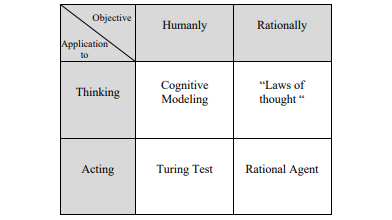
\includegraphics[width=0.7\textwidth]{./figures/ml/ai_streams.png} % Adjust the width to 50% of the text width
%     \caption{AI research streams based on Norvig.}
%     \label{fig:ml_taxonomy}
% \end{figure}

%%%%%%%%%%%%%%%%%%%%%%%%%%%%%%%%%%%%%%%%%%%%%%%%%%%%%%%%%%%%%%%%%%%%%%%%%%%%%%%%%%%%%%%%%%%%%%%%%%%%%%%%%%%%%%%%%%%%%%%%%%%%%%%%%%%%%%%%%%%%%%%%%%%%%%%%%%%%%%
\subsection{The Taxonomy Machine Learning Techniques}
Now that a clear distinction between the terms AI and ML is established, it is crucial to examine the nature of the diverse methodologies encompassed
by ML\@. The generalisability of published research on this issue remains a challenge. Over recent years, various studies have offered differing
classifications of ML methods, with the determining factor being the scope under which ML was investigated. Predominantly, existing literature has been
concentrated on the nature of the feedback mechanism applied, primarily categorizing ML algorithms into supervised, unsupervised and semi-supervised
~\cite{edge_computing_ml_2023, ml_big_data_2019} with some studies also incorporating reinforcement learning into their analysis
~\cite{survey_ml_big_data_2016, sarker_ml_algorithms_2021}.

This research, however, adopts a more holistic approach, aspiring to grasp the whole spectrum of ML applications. Instead of focusing solely on the
nature of the learning feedback, this classification also considers the objectives of the learning tasks and the timing of data availability. This
broader taxonomy, initially introduced by Zhou et al.\cite{zhou_ml_big_data_challenges_2017}, encapsulates all the critical elements that influence
the design and deployment of ML algorithms. The suggested taxonomy is the one shown below in \cref{fig:ml_taxonomy}.

\begin{figure}[!ht]
    \centering
    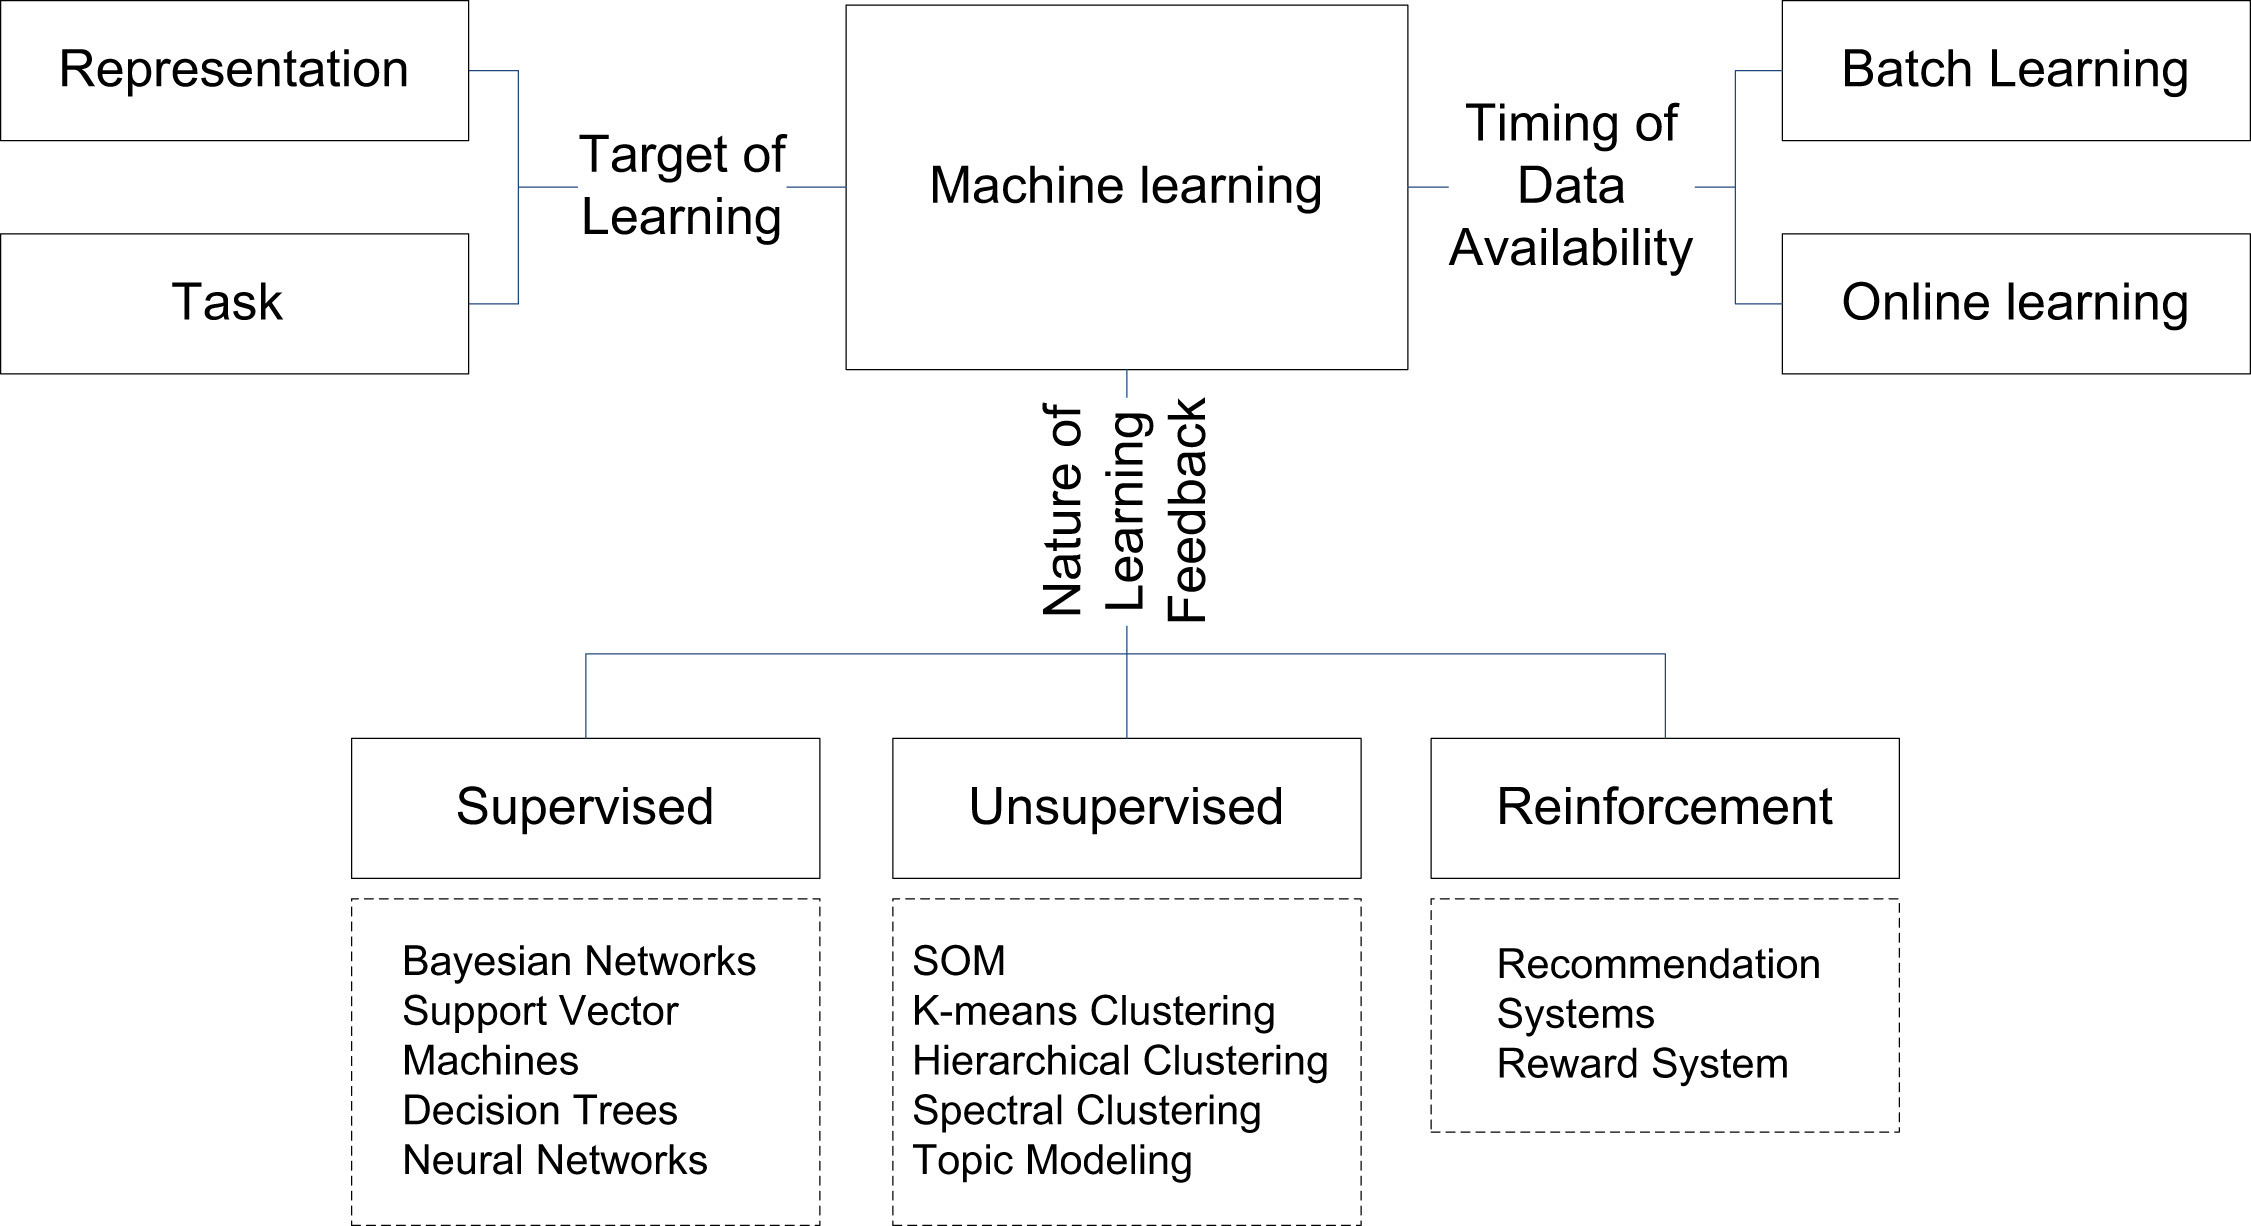
\includegraphics[width=.95\textwidth, keepaspectratio]{./figures/ml/ml_structure.jpg}
    \caption{Multi-dimensional taxonomy of Machine Learning\cite{zhou_ml_big_data_challenges_2017}.}
    \label{fig:ml_taxonomy}
\end{figure}

\begin{itemize}
    \item \textbf{Nature of Learning Feedback:} Based on this dimension of the taxonomy applied to Machine Learning, three principal system categories and one secnondary system
          emerge: supervised, unsupervised, and reinforcement learning systems and semi-supervised (secondary). In supervised learning, sample input-output pairs are presented to the
          system, which in turn attempts to infer a function able to map inputs to corresponding outputs. In practical terms, supervised ML techniques strive
          to construct a predictive model by applying algorithms to a set of known data points to extrapolate insights to an unseen dataset\cite{sarker_ml_algorithms_2021,hastie_statistical_learning_2017}.

          Unsupervised learning, in contrast, can be identified as a more data-driven approach, where datasets devoid of labels are analyzed. This means that while
          the structure of the data is apparent; no explicit guidance is provided as to the expected outcome and the aim is to uncover inherent patterns within
          the data without predefined answers.

          Likewise, reinforcement learning is not provided with input-output pairs, thus resembling unsupervised learning.
          Yet it requires a form of feedback—namely rewards or penalties linked to the actions taken. This environment-driven feedback mechanism guides the
          learning process towards optimal decision-making in an effort to minimize loss or maximize reward, depending on the environment's setup\cite{spyropoulos_lectures_2023}.
          The distinct applications of these techniques are demonstrated by Qiu et al.\cite{survey_ml_big_data_2016}, who assert that supervised and unsupervised
          learning primarily concentrates on data analysis, whereas reinforcement learning is better suited for decision-making tasks.

          Additionally, semi-supervised learning which sits at the intersection of supervised and unsupervised learning, entails learning from a limited set of
          labeled data complemented by a larger pool of unlabeled data. The aim of this learning method is similar to supervised learning, yet the
          knowledge is gathered both from annotated and unannotated data. Some of the key algorithmic examples of each category are demonstrated in the following \cref{table:feedback_taxonomy};

          \begin{table}[h!]
              \centering
              \begin{tabularx}{\textwidth}{>{\hsize=0.7\hsize\arraybackslash}X >{\hsize=1.8\hsize\arraybackslash}X >{\hsize=0.5\hsize\arraybackslash}X}
                  \toprule
                  \rowcolor{lightgray}
                  \textbf{Learning type} & \textbf{Model building}                                & \textbf{Examples}          \\
                  \midrule
                  Supervised             & Algorithms learn from labeled data (task-driven)       & Classification, regression \\
                  Unsupervised           & Algorithms learn from unlabeled data (data-driven)     & Clustering, associations   \\
                  Semi-supervised        & Models built using combined data (labeled + unlabeled) & Classification, clustering \\
                  Reinforcement          & Models based on reward or penalty (environment-driven) & Classification, control    \\
                  \bottomrule
              \end{tabularx}
              \caption{Learning types based on feedback along with key examples of each field}
              \label{table:feedback_taxonomy}
          \end{table}

    \item \textbf{Target of Learning:} Machine learning can be segmented into representational and task learning based on the target of learning—whether
          it focuses on input features or specific tasks respectively. Representational learning seeks to identify novel data representations that simplify
          the extraction of useful information for constructing classifiers or other predictors\cite{bengio_representational_learing_2013}. This approach
          frequently entails isolating critical features that display firm influence upon data variability, which can be proven exceptionally practical in
          probabilistic models aiming to capture the posterior distributions of fundamental factors. Common processes in this category include density
          estimation, which attempts to define the underlying probability density of data and dimensionality reduction, aimed at reducing the complexity
          of data from a higher to a lower-dimensional space. Last but not least, another fundamental example of representational learning is deep learning
          which is one of the fastest-growing fields of ML providing a viable approach for big data processing. All things considered though, defining clear
          objectives in representational learning can be challenging.

          On the contrary, task learning is more outcome-oriented, targeting definite outputs, and can be recognized both in supervised and
          un-supervised setups. To offer an illustration, classification and regression, generally categorized under supervised learning, aim to predict
          discrete classes and continuous values respectively\cite{nastesaki_supervised_ml_2017}, whereas clustering-a form of unsupervised learning-groups
          data without predefined categories\cite{ghahramani_unsupervised_ml_2004}. All things considered, each technique addresses specific analytical needs
          and applications within the broader ML framework.

    \item \textbf{Timing of Data Availability:} On the basis of data availability timing, Machine Learning can be classified into online and batch
          learning. Briefly, batch learning algorithms consolidate knowledge by training comprehensively on the entirety of the dataset available at a certain
          point in time, whereas online learning algorithms process data continuously in streams, accommodating updates through individual samples or
          mini-batches\cite{bisongBatchVsOnline2019}.

          To elucidate these methodologies, in the offline learning scenario typical of batch processing, once
          training is complete and the model is exhibiting adequate performance on the test set, the model is finalized and deployed. In case of new data
          becoming available, indicating a need for model recalibration, a new cycle of training and evaluation needs to be performed integrating both
          existing and new data. Another key factor to note is that the batch learning process functions under the belief that data are Independent and
          Identically Distributed (IID) or that data are drawn from the same probability distribution\cite{dekel_online_to_batch_2008}. Nonetheless, this
          assumption often diverges from the complexities of real-world data dynamics.

          Conversely, online learning operates under no statistical assumptions
          and adapts continuously to data, rendering it indispensable in environments where data generation is ceaseless or complete dataset
          training is impractical. Last but not least, another principal difference between the two ML categorizations is that batch training is expected to
          generalize, producing a more broad reflection of knowledge, while this principle does not uniformly apply to online learning, which focuses on immediate,
          accurate predictions on incoming data data\cite{dekel_online_to_batch_2008}.
\end{itemize}


All things considered, the above multi-dimensional taxonomy can be applied to any given machine learning algorithm, resulting in a categorization along the three
discrete axes displayed at \cref{fig:ml_taxonomy}. For instance, conventional decision trees belong to supervised, task-oriented, batch-learning algorithms.

%%%%%%%%%%%%%%%%%%%%%%%%%%%%%%%%%%%%%%%%%%%%%%%%%%%%%%%%%%%%%%%%%%%%%%%%%%%%%%%%%%%%%%%%%%%%%%%%%%%%%%%%%%%%%%%%%%%%%%%%%%%%%%%%%%%%%%%%%%%%%%%%%%%%%%%%%%%%%%
\subsection{Model Complexity \&\ Challenges}
In an effort to measure the efficiency and generalizability of Machine Learning algorithms, two crucial terms to consider are model performance and complexity.
Model performance refers to the effectiveness of a model in making accurate predictions or decisions based on new, unseen data\cite{perez_model_performance_2022}.
Performance is typically assessed using metrics such as accuracy for classification or mean squared error for regression. For the purposes of this study, accuracy
is the observed metric and can be calculated as follows:

\begin{equation}
    accuracy = \frac{Correct Observations}{Total Observations}
    \label{eq:accuracy}
\end{equation}

In addition to quantifying efficiency, model performance provides a tangible estimator for whether a model is improving or not with new data while enabling different
ML algorithm comparisons under a common scope.

\subsubsection{Model Complexity}
Model complexity relates to a model's ability to represent a wide range of functions, primarily influenced by its architecture,
such as the number of parameters, the depth, and the types of functions it can incorporate. Essentially, complexity determines
the model's capacity to capture intricate patterns within the data. Increasing a model's complexity means introducing more parameters,
thereby enhancing its adaptability to diverse patterns. However, this increase comes at a cost: while the risk of underfitting diminishes,
the danger of overfitting becomes significant, as the model might become excessively tailored to the training dataset, making it too
complex for the data it needs to generalize from\cite{zhang_overfitting_2019,perezModelComplexityMachine2022}.

%%%%%%%%%%%%%%%%%%%%%%%%%%%%%%%%%%%%%%%%%%%%%%%%%%%%%%%%%%%%%%%%%%%%%%%%%%%%%%%
\subsubsection{Balancing Challenges: Overfitting and Underfitting}
\label{sub2:overfitting}
The key to optimizing model performance lies in carefully adjusting its complexity to find a balance between overfitting
and underfitting. Overfitting happens when a model captures not only the underlying patterns but also the noise within the
training data, leading to excellent performance on the training set but poor generalization to new, unseen data
~\cite{zhang_overfitting_2019,sullivanUnderstandingMachineLearning2022}. Conversely, underfitting occurs when the model is
too simplistic, failing to capture the true patterns in the data, which results in suboptimal performance on both the training
and test datasets. This issue often arises when the model lacks sufficient complexity to learn the relationships between input
features and the target variable.

%%%%%%%%%%%%%%%%%%%%%%%%%%%%%%%%%%%%%%%%%%%%%%%%%%%%%%%%%%%%%%%%%%%%%%%%%%%%%%%
\subsubsection{Techniques to Achieve Generalizability}
To find the optimal complexity where the model effectively extracts valuable patterns from the data without overfitting, several techniques are commonly employed:

\begin{itemize}
    \item \emph{Regularization:} This involves adding a penalty term to the loss function to prevent the model from becoming overly complex.
          Techniques like L1 (Lasso) and L2 (Ridge) regularization are widely used to achieve this.
    \item \emph{Cross-validation:} This technique evaluates model performance on unseen data by partitioning the dataset into multiple training
          and validation sets, and averaging the evaluation metrics across all partitions to ensure robust performance.
    \item \emph{Early stopping:} This involves monitoring the model's performance on a validation set during training and halting the training
          process when the performance on the validation set starts to decline, thereby preventing overfitting.
\end{itemize}

These strategies are essential for maintaining the delicate balance between overfitting and underfitting, ensuring that the model remains
generalizable and performs well on new, unseen data\cite{medium_ml_overfitting_2023}.


%%%%%%%%%%%%%%%%%%%%%%%%%%%%%%%%%%%%%%%%%%%%%%%%%%%%%%%%%%%%%%%%%%%%%%%%%%%%%%%
%2
\section{Artificial Neural Networks}
% Artificial Neural Networks (ANNs) represent one of the most dynamic research fields in Machine Learning, forming the backbone of deep learning
% —a subset of machine learning that has revolutionized the handling of vast and complex datasets.
% Their architectural foundation resembles the one of the human brain, which ANNs attempt to mimic. In other words, similar to the
% human brain, ANNs consist of layers of interconnected nodes, otherwise known as "neurons", designed to perform specific computational tasks
% ~\cite{dongare_intro_ANN_2012}.

% Several fields have made great progress by utilizing this architecture—namely, image and speech recognition,
% natural language processing, and decision-making under uncertainty have all benefited massively from the application of Neural Networks.
% These immense capabilities of ANNs transfer admirably to a variety of everyday needs, ranging from healthcare diagnostics to autonomous
% vehicles and financial modeling, showcasing noteworthy robustness and versatility\cite{wu_feng_ANN_development_2018}. However, when regarding
% the ANNs described in this research study under the scope of the previously proposed taxonomy (see \cref{fig:ml_taxonomy}), we will focus on
% online learning ANNs that apply task-oriented supervised learning for classification purposes.

Artificial Neural Networks (ANNs) are a pivotal research area in Machine Learning, forming the backbone of deep learning, which has transformed handling
vast and complex datasets. ANNs mimic the human brain's architecture, consisting of layers of interconnected neurons designed for specific computational
tasks~\cite{dongare_intro_ANN_2012}. ANNs have significantly advanced fields such as image and speech recognition, natural language processing, and
decision-making under uncertainty. Their versatility extends to various applications, including healthcare diagnostics, autonomous vehicles, and financial
modeling, demonstrating robustness and adaptability\cite{wu_feng_ANN_development_2018}. This study focuses on online learning ANNs applying supervised learning
for classification.

%%%%%%%%%%%%%%%%%%%%%%%%%%%%%%%%%%%%%%%%%%%%%%%%%%%%%%%%%%%%%%%%%%%%%%%%%%%%%%%%%%%%%%%%%%%%%%%%%%%%%%%%%%%%%%%%%%%%%%%%%%%%%%%%%%%%%%%%%%%%%%%%%%%%%%%%%%%%%%
\subsection{Perceptron and Activation Functions}
\subsubsection{Rosenblatt and Multi-Layer Perceptrons}

Perceptrons, regarded as one of the earliest and simplest forms of artificial neurons, were initially introduced by Frank Rosenblatt in 1958
~\cite{rosenblattPerceptronProbabilisticModel1958}. Perceptrons functionality is closely related to classification tasks and can be
divided into two categories; Rosenblatt Perceptrons and Multi-Layer Perceptrons (MLP).

The first definition of perceptrons resembles a single-layer neural network with $m$ input sources and one sole output neuron,
where stimuli can be classified into two classes, using a linear decision boundary based on the Heaviside function. This single-layer structure,
restricts Rosenblatt perceptron flexibility, limiting its functionality to linearly separable problems and binary classification tasks. To
demonstrate the functionality of this kind of perceptron, a more strict mathematical description seems necessary\cite{zhangArtificialNeuralNetwork2018}:
\begin{equation}
    % \[
    \begin{cases}
        v = \sum_{i=1}^{m} w_i x_i + b, \\
        y = \phi(v)
    \end{cases}
    % \]
    \label{eq:perceptron}
\end{equation}

Expanding on the definition provided by \cref{eq:perceptron}, Consider $x_i$ (for $i = 1, \ldots, m$) as
the set of input signals delivered to a perceptron. In this model, each $w_i$ represents the synaptic weight associated with the perceptron for
the corresponding input $x_i$. The term $b$ is known as the externally set bias. The term $v$ is referred to as the \emph{induced local field}
or simply the linear combiner of inputs and weights. The function $\phi$, which is an activation function or a step function, processes this induced
local field to produce the output $y$ (see \cref{fig:ros_perceptron}) of the perceptron. This perceptron model essentially consists of a linear
combiner capped by a step function, which decisively determines the output based on the calculated local field $v$.

% \cite{zhangArtificialNeuralNetwork2018} -> rosenblatt_perceptron.jpg
\begin{figure}[!ht]
    \centering
    
\includegraphics[width=.8\textwidth]{./figures/ann/rosenblatt.png}
    \caption{Simple representation of Rosenblatt’s perceptron.}
    \label{fig:ros_perceptron}
\end{figure}

The activation function of Rosenblatt' perceptron, also referred to as the Heaviside step function, is a straightforward threshold function summarized by \cref{eq:heaviside_step}.
The binary output of the function allows us to determine whether an input sample belongs to one out of two classes limiting strictly in binary classification problems
~\cite{popescuMultilayerPerceptronNeural2009}. For this reason, more adaptable activation functions were introduced for various use cases which will be outlined later:

\begin{equation}
    \phi(v) =
    \begin{cases}
        1 & \text{if } v > 0,    \\
        0 & \text{if } v \leq 0.
    \end{cases}
    \label{eq:heaviside_step}
\end{equation}

% Despite the foundational impact of Rosenblatt's perceptrons in the field of neural networks, the limitation encountered in non-linear
% problems created a gap that needed to be filled by a more sophisticated approach. This need led subsequently to the research and development
% of Multi-Layer Perceptron (MLP) Models, similar to the ones utilized today in neural network applications, providing a solution to the famous XOR problem
% initially stated by Marvin Minsky and Seymour Papert in their book\cite{minskyPerceptronsReissue19882017}. Essentially, the incorporation of
% multiple layers of neurons, including hidden ones, opened the gate for learning intricate patterns within the data, enhancing the learning
% capabilities and potential of the systems with non-linear transformations.

% This fundamental advancement in the field enhanced the network's
% generalization ability by learning hierarchical features from the data and improved its flexibility to adapt to different levels of complexity,
% ranging from simple linear problems to problems with complex decision boundaries that single-layer perceptrons could not handle.

% The architecture of a Multi-Layer Perceptron (MLP) differs substantially from Rosenblatt's approach. To be precise, the architecture of the perceptron
% can be divided into three types of layers.

Despite the foundational impact of Rosenblatt's perceptrons in neural networks, their limitations with non-linear problems created a need for a more sophisticated
approach. This led to the development of Multi-Layer Perceptron (MLP) models, which addressed the famous XOR problem highlighted by Marvin Minsky and Seymour
Papert\cite{minskyPerceptronsReissue19882017}. By incorporating multiple layers of neurons, including hidden ones, MLPs can learn intricate patterns in data,
enhancing their learning capabilities and handling non-linear transformations. This advancement improved the network's generalization ability by learning hierarchical
features and adapting to various levels of complexity, from linear problems to complex decision boundaries that single-layer perceptrons could not manage.

The architecture of a Multi-Layer Perceptron (MLP) differs substantially from Rosenblatt's perceptrons. It consists of three types of layers:

\begin{itemize}
    \item \emph{Input layer:} $n$ source neurons.
    \item \emph{Hidden layers:} one or several hidden layers each containing containing \(h_i\) neurons.
    \item \emph{Output layer:} \(m\) output neurons.
\end{itemize}

Each neuron in the network employs a differentiable non-linear activation function. The most commonly utilized activation function in MLPs
is the sigmoid which is close to linear near the origin while saturating rather quickly when getting away\cite{popescuMultilayerPerceptronNeural2009}. This allows multilayer
perceptrons to model well both strongly and mildly nonlinear relations. Additionally, the structure of this MLP is fully connected, meaning every neuron
in a given layer is connected to all neurons in the subsequent layer (see \cref{fig:multi_perceptron}). Signals in the network flow unidirectionally
from the input layer to the output layer, moving sequentially through each layer from left to right.
\begin{figure}[!ht]
    \centering
    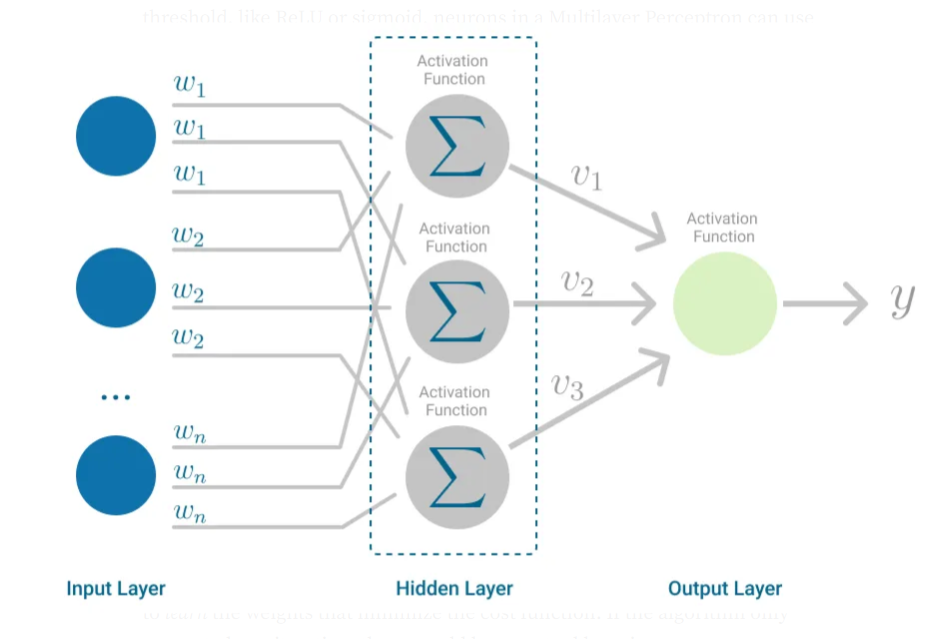
\includegraphics[width=0.75\textwidth, keepaspectratio]{./figures/ann/mlp_2.png}
    \caption{A simple MLP example with $n$ input neurons, one hidden layer with $h_1=3$ neurons and $m=1$ output neuron.}
    \label{fig:multi_perceptron}
\end{figure}




% \cite{zhangArtificialNeuralNetwork2018} -> mlp.png
%%%%%%%%%%%%%%%%%%%%%%%%%%%%%%%%%%%%%%%%%%%%%%%%%%%%%%%%%%%%%%%%%%%%%%%%%%%%%%%
\subsubsection{Evolution of Activation Functions}
The functionality of neural networks is greatly influenced by the choice of activation functions. Initially, Rosenblatt's perceptron used the Heaviside step function,
a basic activation function that activates based on a simple threshold rule.

As neural network theory developed, more flexible activation functions were needed to enable learning in multi-layer architectures and address non-linear classification
problems that single-layer perceptrons could not solve. The sigmoid function emerged as one of the most popular choices for Multi-Layer Perceptrons (MLPs) because of
its continuous and differentiable nature, which is crucial for gradient-based learning algorithms like backpropagation.

Over the years, several other activation functions have been introduced to meet specific requirements of neural network architectures and problems. Common examples
include the hyperbolic tangent (tanh), which is similar to the sigmoid but ranges from -1 to 1, centering the data; the Rectified Linear Unit (ReLU), popular in deep
learning networks due to its efficiency and effectiveness at preventing the vanishing gradient problem\cite{VanishingGradientProblem}; and Softmax, predominantly used
in the output layer of Convolutional Neural Networks (CNNs) to convert logits into a probability distribution over multiple exclusive classes (see \cref{sec:cnn}).

These activation functions have been extensively researched to maximize neural network performance\cite{dubeyActivationFunctionsDeep2022,sharmaACTIVATIONFUNCTIONSNEURAL2020}.
\Cref{table:activation_functions}\footnote{The indexed $v_i$ in Softmax's equation in the table symbolizes the reference to class $i$.}
presents a summary of commonly used activation functions.

\begin{table}[h!]
    \centering
    \begin{tabular}{M{0.15\textwidth} M{0.3\textwidth} M{0.15\textwidth} M{0.3\textwidth}}
        \toprule
        \rowcolor{lightgray}
        \textbf{Function}            & \textbf{Equation}                                                                     & \textbf{Use}              & \textbf{Graph}                                                                      \\
        \midrule
        Heaviside Step               & $\phi(v) = \begin{cases} 1 & \text{if } v > 0 \\ 0 & \text{if } v \leq 0 \end{cases}$ & Binary Classification     & 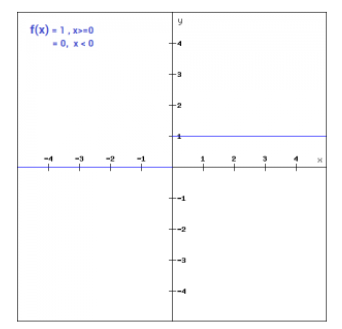
\includegraphics[width=\linewidth, height=25mm]{figures/ann/step_function.png}      \\
        \addlinespace[5pt]
        Sigmoid                      & $\phi(v) = \frac{1}{1 + e^{-v}}$                                                      & Probabilities             & 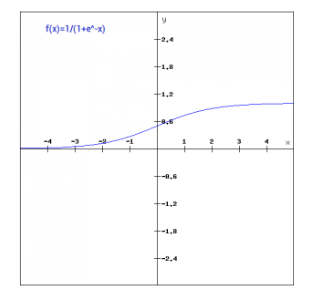
\includegraphics[width=\linewidth, height=25mm]{figures/ann/sigmoid_function.png}   \\
        \addlinespace[10pt]
        Hyperbolic Tangent (tanh)    & $\phi(v) = \frac{e^v - e^{-v}}{e^v + e^{-v}}$                                         & Centered Data             & 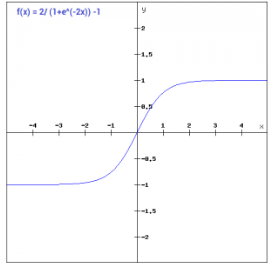
\includegraphics[width=.91\linewidth, height=25mm]{figures/ann/tanh_function.png}   \\
        \addlinespace[10pt]
        Rectified Linear Unit (ReLU) & $\phi(v) = \begin{cases} v & \text{if } v > 0 \\ 0 & \text{if } v \leq 0 \end{cases}$ & Sparse Activation         & 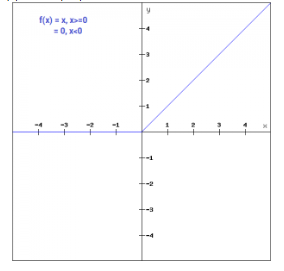
\includegraphics[width=\linewidth, height=25mm]{figures/ann/relu_function.png}      \\
        \addlinespace[10pt]
        Softmax                      & $\phi(v_i) = \frac{e^{v_i}}{\sum_{k} e^{v_k}}$                                        & Multiclass Classification & 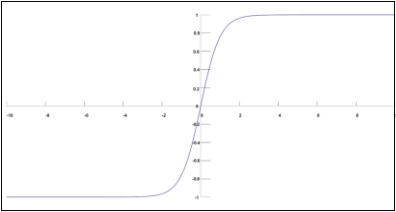
\includegraphics[width=.9\linewidth, height=25mm]{figures/ann/softmax_function.png} \\
        \bottomrule
    \end{tabular}
    \caption{Commonly used activation functions in neural networks\cite{sharmaACTIVATIONFUNCTIONSNEURAL2020}
    }
    \label{table:activation_functions}
\end{table}

These developments have significantly shaped the design and implementation of modern neural networks. The shift from simple threshold functions to complex
non-linear functions has enabled neural networks to model intricate patterns in data, improving their ability to generalize from training data to unseen situations.
This transition marks a pivotal evolution from early perceptrons to the sophisticated networks at the forefront of artificial intelligence research and applications today.



% The functionality of neural networks is greatly influenced by the choice of activation functions. Initially, as with Rosenblatt's perceptron, the $Heaviside$
% step function was the primary activation function used. This simple function determined whether to activate or not based on a simple threshold
% rule.

% As neural network theory developed, the need for more flexible activation functions became apparent, particularly to enable learning in
% multi-layer architectures and to address non-linear classification problems that single-layer perceptrons could not solve. The $sigmoid$ function emerged as one
% of the most popular choices for MLPs because of its continuous and differentiable nature, which is crucial for gradient-based learning algorithms like backpropagation.

% Several other activation functions were introduced in subsequent years depending on the specific requirements of the neural network architecture and the problem at
% hand. Some common examples include the hyperbolic tangent (tanh), which is similar to the sigmoid but ranges from -1 to 1, the Rectified Linear Unit (ReLU),
% which is particularly popular in deep learning networks due to its efficiency and effectiveness at preventing the vanishing gradient problem\cite{VanishingGradientProblem}
% and Softmax, that is predominantly used in the output layer of CNNs (see \cref{sec:cnn}), to convert the logits output into a probability distribution over multiple exclusive
% classes.

% All of the activations
% functions discussed have been thoroughly researched by multiple sources\cite{dubeyActivationFunctionsDeep2022,sharmaACTIVATIONFUNCTIONSNEURAL2020} to examine their
% field of excellence in order to maximize neural network performance. \Cref{table:activation_functions} presents a brief summary.


% \begin{table}[h!]
%     \centering
%     \begin{tabular}{M{0.15\textwidth} M{0.3\textwidth} M{0.15\textwidth} M{0.3\textwidth}}
%         \toprule
%         \rowcolor{lightgray}
%         \textbf{Function}            & \textbf{Equation}                                                                     & \textbf{Use}              & \textbf{Graph}                                                                      \\
%         \midrule
%         Heaviside Step               & $\phi(v) = \begin{cases} 1 & \text{if } v > 0 \\ 0 & \text{if } v \leq 0 \end{cases}$ & Binary Classification     & 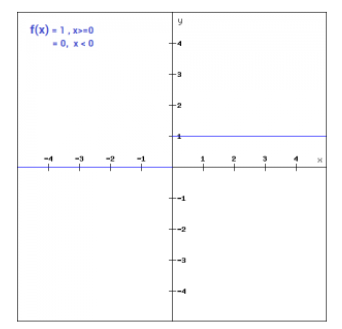
\includegraphics[width=\linewidth, height=25mm]{figures/ann/step_function.png}      \\
%         \addlinespace[5pt]
%         Sigmoid                      & $\phi(v) = \frac{1}{1 + e^{-v}}$                                                      & Probabilities             & 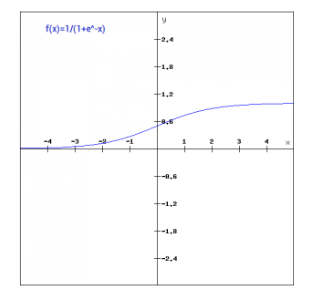
\includegraphics[width=\linewidth, height=25mm]{figures/ann/sigmoid_function.png}   \\
%         \addlinespace[10pt]
%         Hyperbolic Tangent (tanh)    & $\phi(v) = \frac{e^v - e^{-v}}{e^v + e^{-v}}$                                         & Centered Data             & 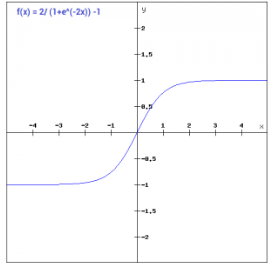
\includegraphics[width=.91\linewidth, height=25mm]{figures/ann/tanh_function.png}   \\
%         \addlinespace[10pt]
%         Rectified Linear Unit (ReLU) & $\phi(v) = \begin{cases} v & \text{if } v > 0 \\ 0 & \text{if } v \leq 0 \end{cases}$ & Sparse Activation         & 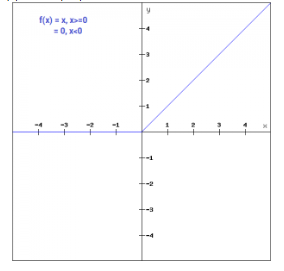
\includegraphics[width=\linewidth, height=25mm]{figures/ann/relu_function.png}      \\
%         \addlinespace[10pt]
%         Softmax                      & $\phi(v_i) = \frac{e^{v_i}}{\sum_{k} e^{v_k}}$                                        & Multiclass Classification & 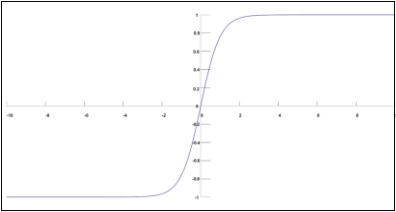
\includegraphics[width=.9\linewidth, height=25mm]{figures/ann/softmax_function.png} \\
%         \bottomrule
%     \end{tabular}
%     \caption{Commonly used activation functions in neural networks\cite{sharmaACTIVATIONFUNCTIONSNEURAL2020}
%         \emph{Comment:} The indexed $v_i$ in Softmax symbolizes the reference to class $i$.}
%     \label{table:activation_functions}
% \end{table}

% These developments have significantly shaped the design and implementation of modern neural networks. The advancement from simple threshold functions
% to complex non-linear functions has enabled neural networks to model intricate patterns in data, improving their ability to generalize from training
% data to unseen situations. This transition marks a pivotal evolution from early perceptrons to the sophisticated networks that are at the forefront
% of artificial intelligence research and applications today.

%%%%%%%%%%%%%%%%%%%%%%%%%%%%%%%%%%%%%%%%%%%%%%%%%%%%%%%%%%%%%%%%%%%%%%%%%%%%%%%%%%%%%%%%%%%%%%%%%%%%%%%%%%%%%%%%%%%%%%%%%%%%%%%%%%%%%%%%%%%%%%%%%%%%%%%%%%%%%%
\subsection{Network Architectures}
The research in the domain of neural networks always strives for optimization, and to be precise, maximization of performance and generalization\cite{ransisiNeuralNetworkTypes2021}.
Hence, in an effort to expand the limits of what can be achieved with Neural Networks, several diverse architectures have been proposed, tailored
for specific data and fields. That way performance is improved by addressing the specific needs of a given problem. While the types of architectures
developed to this day are countless, this analysis will be restricted to a brief overview of two major categories and afterward, there will be a shift in focus
toward the architecture most valuable for this research.

\begin{figure}[h!]
    \centering
    \begin{subfigure}[t]{0.49\textwidth}
        \centering
        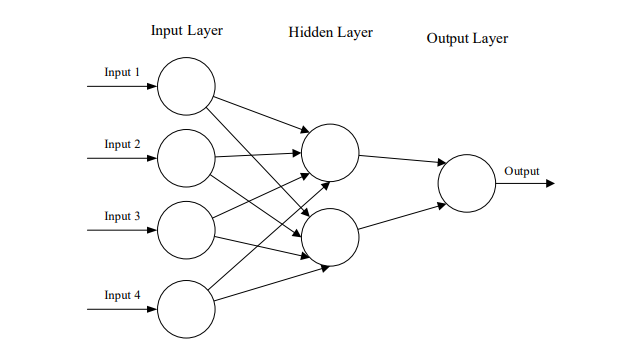
\includegraphics[width=1.1\textwidth,height=.6\textwidth]{figures/ann/ffnn.png}
        \caption{FFNN with one hidden layer\cite{osheaIntroductionConvolutionalNeural2015}.}
        \label{fig:ffnn}
    \end{subfigure}\hfill
    \begin{subfigure}[t]{0.49\textwidth}
        \centering
        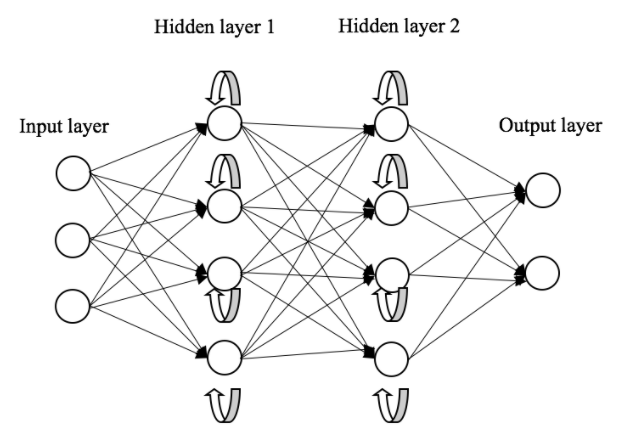
\includegraphics[width=\textwidth]{figures/ann/rnn1.png}
        \caption{General structure of RNNs\cite{communityUnderstandingMechanismTypes2020}.}
        \label{fig:rnn}
    \end{subfigure}
    \caption{A side by side illustration of FFNN and RNN architectures.}
    \label{fig:ffnn_rnn}
\end{figure}

First and foremost, there are Feed-Forward Neural Networks (FFNN)\cite{leshnoMultilayerFeedforwardNetworks1993} which represents the simplest form of
neural network, designed on the tracks of MLPs' logic discussed previously (see \cref{fig:ffnn}). In this type of networks, neurons are organized
in layers with each neuron being connected to all neurons of subsequent layers. The network's flow is unidirectional from the input layer through hidden
layers to the output layer. Common use examples contain image and speech recognition, due to their simplicity and effectiveness.

Moving forward, another crucial type of neural network architecture is Recurrent Neural Networks (RNNs)\cite{communityUnderstandingMechanismTypes2020}.
Recurrent Neural Networks are designed to handle sequential data\cite{ghiassiDynamicArtificialNeural2005}. Differing from traditional neural networks, RNNs process inputs
using a loop mechanism that allows information from previous steps to influence current and future operations (see \cref{fig:rnn}). This architecture
~\cite{osheaIntroductionConvolutionalNeural2015} makes RNNs ideal for applications such as language modeling and text generation, where the sequence and context
of information are critical. They are particularly effective in tasks like speech recognition, music generation, and other forms of sequential pattern recognition.

%%%%%%%%%%%%%%%%%%%%%%%%%%%%%%%%%%%%%%%%%%%%%%%%%%%%%%%%%%%%%%%%%%%%%%%%%%%%%%%
\subsubsection{Convolutional Neural Networks (CNNs)}
\label{sec:cnn}
% Building on the foundational principles laid out by Feed-Forward Neural Networks, the exploration into network architectures takes a sophisticated turn
% with Convolutional Neural Networks (CNNs)\cite{guRecentAdvancesConvolutional2018}, arguably one of the most significant achievements of Deep Learning.
% CNNs have known great applicability in several fields including image and video recognition, recommendation systems, image classification, image
% segmentation natural language processing, and computer vision. The name of CNNs stems from the \emph{convolution}-an operation described in calculus,
% as a mathematical operation that combines two functions to produce a third, that expresses how the shape of one is modified by the other.
% This inherent property of convolutional layers provides CNNs with translation-invariance, enabling them to detect and extract patterns and
% features from data regardless of changes in position, orientation, scale, or translation.

Building on the foundational principles of Feed-Forward Neural Networks, the exploration into network architectures takes a sophisticated turn with Convolutional
Neural Networks (CNNs)\cite{guRecentAdvancesConvolutional2018}, a significant achievement in Deep Learning. CNNs have broad applicability in fields such as image
and video recognition, recommendation systems, image classification, image segmentation, natural language processing, and computer vision. The name of CNNs stems
from the \emph{convolution}-an mathematical operation described in calculus that combines two functions to produce a third, that expresses how the shape of one
is modified by the other. This inherent property of convolutional layers provides CNNs with translation-invariance, enabling them to detect and extract patterns and features
from data regardless of position, orientation, scale, or translation.

\begin{figure}[!ht]
    \centering
    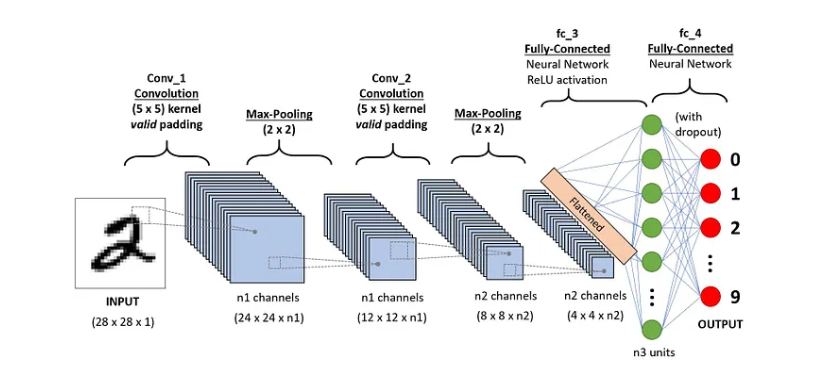
\includegraphics[width=\textwidth]{figures/ann/cnn1.png}
    \caption{A CNN sequence to classify handwritten digits\cite{sahaComprehensiveGuideConvolutional2022}}
    \label{fig:cnn}
\end{figure}

To further elucidate the methodology of a CNN, we will observe the example of \cref{fig:cnn} depicting a single input from the MNIST dataset\footnote{Dataset of handwritten digits}
while being processed. The format in which the system perceives the input is a pixel representation of the image. After the input is received the sample
undergoes a series of critical operations that eventually lead to the system's output.


The \emph{convolution layer} performs a sliding window function to the matrix of pixels representing the digit's image, commonly known as kernel or filter.
Several filters of equal size are applied, and each filter is used to recognize a specific pattern from the image, generating multiple feature maps.
Observing \cref{fig:cnn}, a $4(height)x4(breadth)$ kernel is utilized, sliding over the input image, calculating the convolution result at each point
and populating the feature map.

\begin{figure}[!ht]
    \centering
    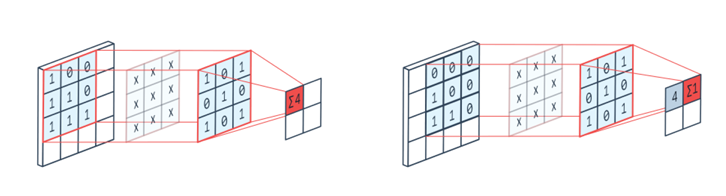
\includegraphics[width=1\textwidth,keepaspectratio]{figures/ann/convolutional_layer.png}
    \caption{A convolution of a $4\times4$ image with a $3\times3$ kernel highlighting the sliding window operation\cite{petrakosemmanouelReconfigurableLogicFPGA2023}}
    \label{fig:kernel}
\end{figure}

After each convolution operation, a ReLU (see \cref{table:activation_functions}) activation function is applied to
deduce non-linear relationships between the features in the image, hence improving the network's capability for
capturing complex patterns.

Following the convolution and activation steps, the \emph{pooling (or subsampling) layer} reduces the spatial dimensions of the feature maps. This step is crucial as it
decreases computational requirements and the number of parameters, helping prevent overfitting. Max pooling, which selects the maximum value from each patch of the
feature map, is the most frequently used method (\cref{fig:max_pooling}). Another common method is average pooling, which calculates the average value of each patch (\cref{fig:avg_pooling}).
The final pooling layer converts the feature map into a flattened, one-dimensional array, preparing it for input into the fully connected layer.

\begin{figure}[!ht]
    \centering
    \begin{subfigure}[b]{0.49\textwidth}
        \centering
        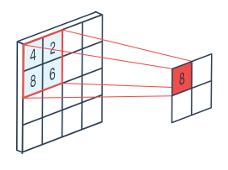
\includegraphics[width=.6\textwidth]{figures/ann/max_pooling.png}
        \caption{Max pooling}
        \label{fig:max_pooling}
    \end{subfigure}
    \hfill
    \begin{subfigure}[b]{0.49\textwidth}
        \centering
        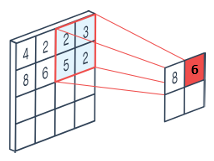
\includegraphics[width=.58\textwidth]{figures/ann/avg_pooling.png}
        \caption{Average pooling}
        \label{fig:avg_pooling}
    \end{subfigure}
    \caption{Demosntration of max and avergae pooling operations.}
    \label{fig:max_and_avg_pooling}
\end{figure}


The \emph{fully connected layers} represent the last layer of a CNN and their inputs correspond to the flattened one-dimensional matrix generated by the last pooling layer.
ReLU activations functions are applied to them for non-linearity again (as shown in \cref{fig:cnn}).
Finally, a softmax prediction layer is used to generate probability values for each of the possible output labels, and the final label predicted is the one with
the highest probability score.
%%%%%%%%%%%%%%%%%%%%%%%%%%%%%%%%%%%%%%%%%%%%%%%%%%%%%%%%%%%%%%%%%%%%%%%%%%%%%%%
%%%%%%%%%%%%%%%%%%%%%%%%%%%%%%%%%%%%%%%%%%%%%%%%%%%%%%%%%%%%%%%%%%%%%%%%%%%%%%%%%%%%%%%%%%%%%%%%%%%%%%%%%%%%%%%%%%%%%%%%%%%%%%%%%%%%%%%%%%%%%%%%%%%%%%%%%%%%%%
\subsection{Learning in Neural Networks}
Having established the principal components and architecture of ANNs, we proceed with a brief demonstration of their learning method.
Learning in neural networks, achieved by training\footnote{Training is also called fitting in ML terminology}, involves the adjustment of the network’s
internal parameters to minimize the discrepancy between the actual output and the target output. This process is crucial for developing models that
can perform well on unseen data. Yet, In order to successfully grasp the reasoning behind the training process, it is crucial to decompose the procedure into
smaller, comprehensive, sub-processes.\cite{martyNeuralNetworksLearning2023}. In essence, this analysis partitions the training process into six parts as follows;

\begin{enumerate}
    \item \emph{Initialization:} The initialization of weights is a critical first step in the training of neural networks. Proper initialization sets the stage for
          an efficient and effective learning process, influencing how quickly a network converges to a solution, if at all. Initially, weights can be set randomly,
          but more sophisticated methods such as He initialization or Xavier initialization are commonly used to improve the convergence properties of deep networks\cite{goodfellowDeepLearning2016}.
          These methods adjust the scale of the weights according to the number of input and output neurons, promoting an even
          distribution of activations across layers during the initial phases of training\cite{narkhedeReviewWeightInitialization2022}.

    \item \emph{Forward Propagation:} This step involves computing the output of a neural network, starting by feeding the input data and calculating the weighted
          sum of each neuron's inputs. The activation or non-activation of the neuron is determined by the output of the nonlinear activation function (see \cref{table:activation_functions})
          over the calculated sum. The process begins at the input layer and proceeds sequentially through the hidden layers and finally to the output layer, where a
          prediction is made. The specific transformations applied to the neurons' sums depend on the network's architecture (e.g., convolutional, recurrent) and the types
          of layers used\cite{nielsenNeuralNetworksDeep}.

    \item \emph{Loss Computation:} A cost (or loss) function, quantifies the error between the predicted outputs and the actual target values.
          The cost function selection can significantly affect the network's performance and convergence. Common choices include Mean Squared Error (MSE) for regression
          tasks and Cross-Entropy Loss for classification tasks. The cost function provides a performance measure used during backpropagation to adjust the model’s weights.

    \item \emph{Back Propagation:} Backpropagation is the fundamental algorithm for training artificial neural networks. It calculates the gradients of the loss function
          with respect to the weights of the network by applying the chain rule of calculus. These gradients indicate the necessary adjustments to the weights to
          minimize the loss function and improve model accuracy. The process involves propagating the error backward through the network, updating the weights to
          reduce the prediction error for subsequent iterations\cite{cilimkovicNeuralNetworksBack}.

    \item \emph{Gradient Descent:} The gradients calculated during the \textit{back propagation phase} comprise a clear indication of the steepest ascent
          on the loss curve, meaning the direction of the maximizing loss. On the contrary, as the objective is to minimize the loss, it becomes obvious that the
          required update of the network’s parameters needs to be performed moving in the opposite direction of the gradients. By iteratively adjusting the weights
          in this direction, the accuracy of the system increases, while The magnitude of this update is controlled by a learning rate hyperparameter of the
          optimization algorithm. Additional information for this matter will be presented in the following \cref{sec:optimization}.

    \item \emph{Iteration:} Steps $2-5$ are repeated for each batch of training data for multiple epochs\footnote{Epoch is a complete pass over the training dataset} until
          the neural network’s performance on the training data achieves convergence to a solution.

\end{enumerate}

The above process is repeated iteratively until the breaking condition is satisfied. However,
this does not necessarily guarantee generalization. The above statement loops back to a previously reported
issue in machine-learning-overfitting (see \cref{sub2:overfitting}). Therefore, training can include a validation
step where the model is tested on unseen data to adjust hyperparameters and prevent overfitting.

In closing analysis, it should be noted that the neural networks, as demonstrated, accumulate knowledge
by iterative adjusting the network's parameters based on the optimization algorithm applied.
This suggests that a vast number of operations need to be performed at each training step.
In restricted-size models, the above operation may be a manageable load for the computers to handle,
then again this is not the fact, for substantially sized networks, where the computational demands can become
humongous. Hence, training neural networks is typically performed on powerful hardware or specialized hardware
accelerators (GPUs or TPUs) to speed up the process\cite{martyNeuralNetworksLearning2023}.

%%%%%%%%%%%%%%%%%%%%%%%%%%%%%%%%%%%%%%%%%%%%%%%%%%%%%%%%%%%%%%%%%%%%%%%%%%%%%%%%%%%%%%%%%%%%%%%%%%%%%%%%%%%%%%%%%%%%%%%%%%%%%%%%%%%%%%%%%%%%%%%%%%%%%%%%%%%%%%

%%%%%%%%%%%%%%%%%%%%%%%%%%%%%%%%%%%%%%%%%%%%%%%%%%%%%%%%%%%%%%%%%%%%%%%%%%%%%%%
%3
\section{Optimization Techniques}
\label{sec:optimization}
Optimization is, undoubtedly, a crucial matter in the field of Data Science and Machine Learning. This section explores various
techniques stemming from optimization theory, aiming to enhance the performance of machine learning algorithms through the effective
minimization of loss functions. Starting from the fundamental principles of Gradient Descent, and continuing by presenting the key
variations relevant to this research approach, this analysis clarifies the role of optimizers in contemporary neural networks.

%%%%%%%%%%%%%%%%%%%%%%%%%%%%%%%%%%%%%%%%%%%%%%%%%%%%%%%%%%%%%%%%%%%%%%%%%%%%%%%%%%%%%%%%%%%%%%%%%%%%%%%%%%%%%%%%%%%%%%%%%%%%%%%%%%%%%%%%%%%%%%%%%%%%%%%%%%%%%%
\subsection{Gradient Descent And Its Variants}
\subsubsection{Principle of Gradient Descent}
Gradient Descent and its Variants are classified as iterative optimization algorithms, based on the idea of iteratively adjusting
the parameters (coefficients) of a model in the direction of the steepest descent with respect to the machine learning algorithm’s
cost function\cite{ruderOverviewGradientDescent2017}. Essentially, the objective of the algorithm is to find the parameter values
that minimize the cost function of the neural network. For this to be achieved, the gradient of the loss function at the current
point is calculated, indicating how small changes in the weights affect its output. Thus, the parameters are iteratively adjusted
in the opposite direction of the gradient—towards the minima point of the cost curve (see \cref{fig:gradient_descent}).

\begin{figure}[!ht]
    \centering
    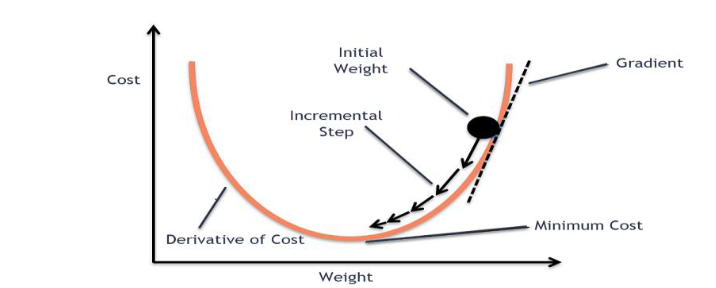
\includegraphics[width=.8\textwidth]{figures/opt/gradient_descent.png}
    \caption{Gradient Descent Algorithm\cite{hajiCOMPARISONOPTIMIZATIONTECHNIQUES2021}}
    \label{fig:gradient_descent}
\end{figure}

%%%%%%%%%%%%%%%%%%%%%%%%%%%%%%%%%%%%%%%%%%%%%%%%%%%%%%%%%%%%%%%%%%%%%%%%%%%%%%%
\subsubsection{Batch Gradient Descent}
Batch Gradient Descent (BGD), also referred to as Vanilla, computes the cost function with regard to the parameters $\theta$ for the
entire training dataset:
\begin{equation}
    \label{eq:bgd}
    \theta_{new} = \theta_{old} - \eta \cdot \nabla_{\theta} J(\theta)
\end{equation}

\noindent
Here, $\theta$ represents the parameters of the function to be minimized, $J(\theta)$ is the loss function, $\nabla_{\theta} J(\theta)$
denotes the gradient of the loss function with respect to $\theta$, and $\eta$ is the learning rate, which controls the size of the incremental
step taken towards the minimum.

Despite being easy to comprehend, BGD requires computing gradients for the entire dataset to update the model once, making it inefficient
for very large datasets or those exceeding memory capacity\cite{ruderOverviewGradientDescent2017}. Additionally, this method does not
support online updates with new data as it processes. Nonetheless, batch gradient descent is guaranteed to converge to the global minimum
for convex error surfaces and to a local minimum for non-convex surfaces.

%%%%%%%%%%%%%%%%%%%%%%%%%%%%%%%%%%%%%%%%%%%%%%%%%%%%%%%%%%%%%%%%%%%%%%%%%%%%%%%
\subsubsection{Stochastic Gradient Descent}
Proceeding with Stochastic Gradient Descent (SGD), this optimization method updates parameters incrementally for each training sample, $x^{(i)}$
and label $y^{(i)}$, unlike the previous discussion regarding BGD\@.

\begin{equation}
    \label{eq:sgd}
    \theta_{new} = \theta_{old} - \eta \cdot \nabla_{\theta} J(\theta; x^{(i)}; y^{(i)})
\end{equation}

The term stochastic in the name refers to the random selection of one sample for the gradient calculation instead of the entirety
of the dataset. This approach has been proven particularly beneficial for large-scale datasets and online learning algorithms as
it aids in reducing training time. Other commonly discussed properties of SGD include the ability to effectively escape local minima,
improved model generalizability to unseen data, and the detailed rate of improvement due to the frequency of updates. At the same time,
this per-sample frequency of parameter updates also leads to fluctuations in the error rate, instead of a steady and controlled decrease.

%%%%%%%%%%%%%%%%%%%%%%%%%%%%%%%%%%%%%%%%%%%%%%%%%%%%%%%%%%%%%%%%%%%%%%%%%%%%%%%
\subsubsection{Mini-Batch Gradient Descent}
This approach of optimization fills the middle space between BGD and SGD, as Mini-Batch Gradient Descent (MBGD) strikes a balance
between the computational efficiency of the former and the stability of the latter. Instead of updating parameters using all or
only one of the training examples, Mini-Batch Gradient Descent uses a subset of \emph{n} training data to perform each update:

\begin{equation}
    \label{eq:mbgd}
    \theta_{new} = \theta_{old} - \eta \cdot \nabla_{\theta} J(\theta; x^{(i:i+n)}; y^{(i:i+n)})
\end{equation}

This approach reduces the variance of the parameter updates, which can lead to more stable convergence than SGD while being
significantly faster than using the full dataset as in Batch Gradient Descent. This method is particularly effective for training
on large datasets making use of highly optimized matrix operations common to state-of-the-art deep learning libraries, resulting
in great efficiency while computing the gradients. All the above have contributed greatly to making MBGD the first choice of
optimization when training neural networks, while sometimes this is the case even when SGD is reported as the optimization algorithm
as the term SGD is used also when mini-batches are employed.

%%%%%%%%%%%%%%%%%%%%%%%%%%%%%%%%%%%%%%%%%%%%%%%%%%%%%%%%%%%%%%%%%%%%%%%%%%%%%%%
%%%%%%%%%%%%%%%%%%%%%%%%%%%%%%%%%%%%%%%%%%%%%%%%%%%%%%%%%%%%%%%%%%%%%%%%%%%%%%%%%%%%%%%%%%%%%%%%%%%%%%%%%%%%%%%%%%%%%%%%%%%%%%%%%%%%%%%%%%%%%%%%%%%%%%%%%%%%%%
\subsection{Towards ADAM Optimizer}

\subsubsection{Learning Rate Selection}
The learning rate hyperparameter, often denoted as $\eta$, is undoubtedly one of the most crucial factors contributing to the
convergence of gradient-based optimization algorithms\cite{ruderOverviewGradientDescent2017}. It determines the incremental step
size of the algorithm towards the minimum of the cost function, as observed in \cref{fig:gradient_descent}. The importance of
balancing the hyperparameter's value cannot be overstated; too high a learning rate can cause the algorithm to overshoot the minimum,
while too low a learning rate can result in excessively slow convergence or getting stuck in local minima (see \cref{fig:learning_rate}).
Therefore, achieving balance in this situation suggests swift convergence to the minimum.

\begin{figure}[!ht]
    \centering
    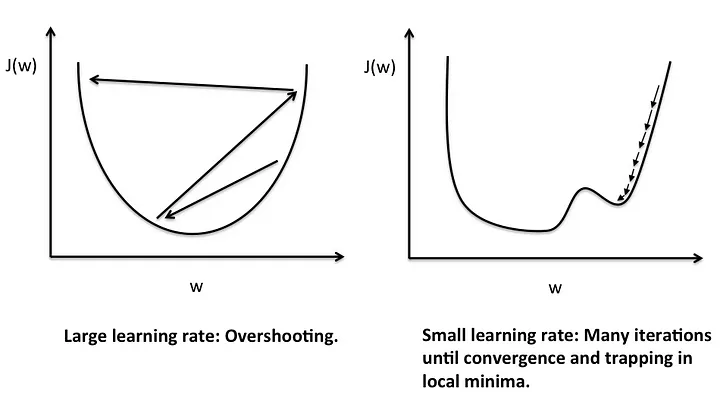
\includegraphics[width=.85\textwidth]{figures/opt/learning_rates_1.png}
    \caption{The effects of unsuccessful learning rate selection\cite{atulanandGRADIENTDESCENT2022}}
    \label{fig:learning_rate}
\end{figure}

%%%%%%%%%%%%%%%%%%%%%%%%%%%%%%%%%%%%%%%%%%%%%%%%%%%%%%%%%%%%%%%%%%%%%%%%%%%%%%%
\subsubsection{Momentum}
Momentum is an enhancement of Gradient Descent that accelerates convergence, particularly in the context of deep neural networks.
The term finds great applicability in situations where the network is not well-conditioned, leading to the composition of \emph{ravines}
—surfaces that curve more steeply in one direction than in another direction\cite{MomentumLearningRate,hajiCOMPARISONOPTIMIZATIONTECHNIQUES2021}.
Such surfaces negatively impact convergence, due to the simple fact that the gradient does not point towards the minimum, and successive
steps of gradient descent can oscillate from one side to the other, progressing, albeit very slowly, to the minimum. \Cref{fig:momentum}
illustrates how the addition of momentum aids in speeding up convergence to the minimum by damping these oscillations.

\begin{figure}[!ht]
    \centering
    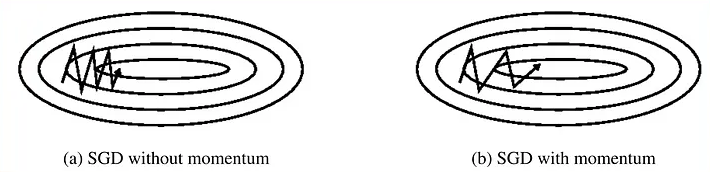
\includegraphics[width=.85\textwidth]{figures/opt/momentum.png}
    \caption{Trajectories in ravine surfaces, with and without momentum\cite{lecunEfficientBackProp1998}.}
    \label{fig:momentum}
\end{figure}

In the formal mathematical representation of SGD Momentum in \cref{eq:momentum}, $v_{t}$ represents the velocity, $\beta$ is the momentum
coefficient (typically set between 0.9 and 0.99), and $\nabla_{\theta} J(\theta; x^{(i)}; y^{(i)})$ is the gradient of the loss function.
In other words, the velocity that is calculated for a given moment $t$ complements the gradient descent calculation by taking into account
the momentum $\beta v_{t-1}$. This way, the update on the network's parameters is computed utilizing the velocity term that includes both
gradient and momentum.
\begin{equation}
    \begin{cases}
        v_{t} = \underbrace{\beta v_{t-1}}_{\text{momentum}} - \underbrace{\eta \cdot \nabla_{\theta} J(\theta; x^{(i)}; y^{(i)})}_{\text{gradient descent}} & \triangleright\text{ Velocity computation} \\
        \theta_{t} = \theta_{t-1} + v_{t}                                                                                                                    & \triangleright\text{ Parameters' update}
    \end{cases}
    \label{eq:momentum}
\end{equation}

%%%%%%%%%%%%%%%%%%%%%%%%%%%%%%%%%%%%%%%%%%%%%%%%%%%%%%%%%%%%%%%%%%%%%%%%%%%%%%%
\subsubsection{ADAM Optimizer}\label{sec:adam}
THe ADAM (Adaptive Moment Estimation) optimizer, proposed by Kingma and Ba (2017)\cite{kingmaAdamMethodStochastic2017}, is a widely utilized algorithm that combines
the benefits of both momentum and
adaptive learning rates, classifying it as an adaptive learning algorithm. This approach leverages concepts from Adagrad\cite{duchiAdaptiveSubgradientMethods}
and RMSprop\cite{LectureRmspropDivide}, making it particularly effective for deep neural network (DNN) training by managing
sparse gradients and non-stationary objectives.

By maintaining exponentially decaying averages, ADAM calculates adaptive learning rates of past gradients and squared gradients.
These moving averages smooth out noise in the gradient updates, providing a stable convergence path.
The momentum aspect, derived from the average of past gradients, helps accelerate convergence by maintaining
consistent update directions, thus reducing oscillations. Its implementation is summarized by \cref{alg:adam}:

In the following steps, $m_t$ and $v_t$ represent the first moment (mean) and second moment (uncentered variance) of the gradients,
respectively. The corrected estimates, $\hat{m}_t$ and $\hat{v}_t$, are used to compute the parameter updates. The decay rates $\beta_1$
and $\beta_2$ are typically set to 0.9 and 0.999, respectively, with $\epsilon$ preventing division by zero.

ADAM's ability to adaptively adjust learning rates for each parameter, based on the mean and variance of gradients, ensures robust performance
across various machine learning applications. This is especially beneficial for hyperparameter tuning and managing high-dimensional loss landscapes.

\begin{algorithm}[H]
    \caption{ADAM optimizer algorithm}
    \label{alg:adam}
    \begin{algorithmic}
        \Require $\alpha$: Stepsize
        \Require $\beta_1, \beta_2 \in [0, 1)$: Exponential decay rates for the moment estimates
        \Require $f(\theta)$: Stochastic objective function with parameters $\theta$
        \Require $\theta_0$: Initial parameter vector
        \Statex
        \Statex \textbf{Initialize:}
        \Statex $m_0 \leftarrow 0$ \Comment{Initialize 1\textsuperscript{st} moment vector}
        \Statex $v_0 \leftarrow 0$ \Comment{Initialize 2\textsuperscript{nd} moment vector}
        \Statex $t \leftarrow 0$ \Comment{Initialize timestep}
        \Statex
        \While{$\theta_t$ not converged}
        \Statex $t \leftarrow t + 1$
        \Statex $g_t \leftarrow \nabla_{\theta} f_t(\theta_{t-1})$ \Comment{Get gradients w.r.t.\ stochastic objective at timestep $t$}
        \Statex $m_t \leftarrow \beta_1 \cdot m_{t-1} + (1 - \beta_1) \cdot g_t$ \Comment{Update biased first moment estimate}
        \Statex $v_t \leftarrow \beta_2 \cdot v_{t-1} + (1 - \beta_2) \cdot g_t^2$ \Comment{Update biased second raw moment estimate}
        \Statex $\hat{m}_t \leftarrow m_t / (1 - \beta_1^t)$ \Comment{Compute bias-corrected first moment estimate}
        \Statex $\hat{v}t \leftarrow v_t / (1 - \beta_2^t)$ \Comment{Compute bias-corrected second raw moment estimate}
        \Statex $\theta_t \leftarrow \theta{t-1} - \alpha \cdot \hat{m}_t / (\sqrt{\hat{v}_t} + \epsilon)$ \Comment{Update parameters}
        \EndWhile
        \Statex \textbf{return} $\theta_t$ \Comment{Resulting parameters}
    \end{algorithmic}
\end{algorithm}

In the Federated Learning realm that is studied, ADAM's optimization techniques are crucial for enhancing convergence rates and model performance.
The decentralized nature of Federated Learning introduces challenges such as heterogeneous data distributions and communication constraints, as will be
discussed in subsequent sections.
ADAM's adaptive learning rate mechanism facilitates effective training across distributed nodes, overcoming data variability and ensuring
efficient global model convergence.
%%%%%%%%%%%%%%%%%%%%%%%%%%%%%%%%%%%%%%%%%%%%%%%%%%%%%%%%%%%%%%%%%%%%%%%%%%%%%%%
%%%%%%%%%%%%%%%%%%%%%%%%%%%%%%%%%%%%%%%%%%%%%%%%%%%%%%%%%%%%%%%%%%%%%%%%%%%%%%%%%%%%%%%%%%%%%%%%%%%%%%%%%%%%%%%%%%%%%%%%%%%%%%%%%%%%%%%%%%%%%%%%%%%%%%%%%%%%%%

%%%%%%%%%%%%%%%%%%%%%%%%%%%%%%%%%%%%%%%%%%%%%%%%%%%%%%%%%%%%%%%%%%%%%%%%%%%%%%%
%4
\section{Distributed Machine Learning}
%%%%%%%%%%%%%%%%%%%%%%%%%%%%%%%%%%%%%%%%%%%%%%%%%%%%%%%%%%%%%%%%%%%%%%%%%%%%%%%%%%%%%%%%%%%%%%%%%%%%%%%%%%%%%%%%%%%%%%%%%%%%%%%%%%%%%%%%%%%%%%%%%%%%%%%%%%%%%%
\subsection{The Need for Distribution}
As the field of machine learning (ML) continues to evolve, the demand for processing vast amounts of data and training
increasingly complex models has surged. Traditional machine-learning methodologies, which typically operate on single-machine setups,
face significant limitations in terms of computational power and memory capacity. This led, in the past, to the development and adoption of
centralized learning approaches, where data from various sources is aggregated into a central location for processing. While centralized
learning mitigates some of the constraints of single-machine learning, it still struggles with issues such as data transfer overhead,
security risks, and the inability to scale efficiently with ever-growing datasets.

To overcome these shortcomings, the paradigm has shifted towards Distributed Machine Learning (DML). DML allows for the distribution of data
and computational tasks across multiple machines or devices, leveraging their collective resources. This approach not only enhances
computational efficiency through parallelism, but also enables the processing of larger datasets that would be infeasible for centralized systems.
By distributing the workload, DML restricts data transfer bottlenecks, enhances fault tolerance, and provides greater scalability, making it an essential
advancement for modern machine learning applications.


\begin{figure}[!ht]
    \centering
    \begin{subfigure}[b]{0.49\textwidth}
        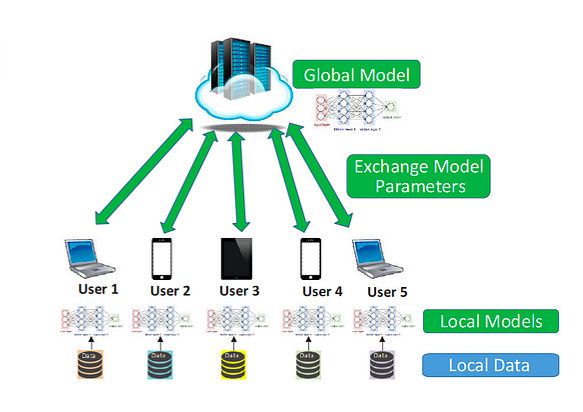
\includegraphics[height=.8\textwidth,keepaspectratio]{figures/dml/distributed_1.png}
        \caption{Distributed Learning}
        \label{fig:distributed}
    \end{subfigure}
    \hfill
    \begin{subfigure}[b]{0.49\textwidth}
        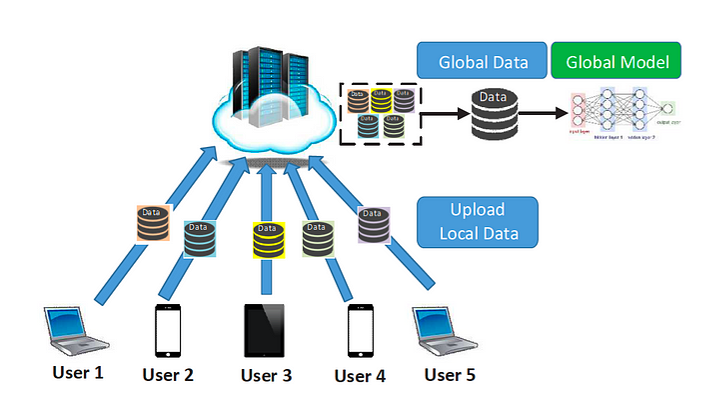
\includegraphics[height=.8\textwidth,keepaspectratio]{figures/dml/centralized.png}
        \caption{Centralized Learning}
        \label{fig:centralized}
    \end{subfigure}
    \caption{A comparison between distributed and centralized learning approaches}
    \label{fig:centralized_vs_distributed}
\end{figure}

Thus, the progression from traditional ML to centralized learning, and finally to DML, reflects the ongoing need to optimize and scale
machine learning processes to keep pace with the increasing data demands and computational complexities of contemporary applications.
%%%%%%%%%%%%%%%%%%%%%%%%%%%%%%%%%%%%%%%%%%%%%%%%%%%%%%%%%%%%%%%%%%%%%%%%%%%%%%%
%%%%%%%%%%%%%%%%%%%%%%%%%%%%%%%%%%%%%%%%%%%%%%%%%%%%%%%%%%%%%%%%%%%%%%%%%%%%%%%%%%%%%%%%%%%%%%%%%%%%%%%%%%%%%%%%%%%%%%%%%%%%%%%%%%%%%%%%%%%%%%%%%%%%%%%%%%%%%%
\subsection{Distributed Learning Systems Architecture}
\label{sec:dml_architecture}
The architecture of DML Systems can be defined by a triad of layers dependent on each other: \emph{The Distribution Method (Parallelism)},
\emph{the System's Communication Topology}, and \emph{the ML algorithm}. A broad overview of the above will be presented as follows:

%%%%%%%%%%%%%%%%%%%%%%%%%%%%%%%%%%%%%%%%%%%%%%%%%%%%%%%%%%%%%%%%%%%%%%%%%%%%%%%
\subsubsection{Parallelism in Distributed Learning Systems}\label{sec:parallelism}
Parallelism in DML Systems can be achieved with two methods; Data and Model Parallelism.
A thorough survey by Joost Verbraeken et al.\cite{joostverbraekenSurveyDistributedMachine} clarifies:
\begin{itemize}
    \item \emph{Data Parallelism:} In the data-parallel approach, the dataset is divided into segments corresponding to the number of worker nodes
          in the system. Each worker node then processes its respective data segment using the same algorithm. The model is either centralized or replicated
          across all worker nodes, ensuring a unified output. This method is applicable to any machine learning algorithm that assumes independent and
          identical distribution (i.i.d.) of data samples, which includes the majority of ML algorithms.

    \item \emph{Model Parallelism:} Model parallelism involves splitting the model itself across multiple machines and training different parts of the model
          on different machines. This approach is useful when the model is too large to fit in the memory of a single machine, or when certain parts of the model
          require more computation than others. Model parallelism is a bit more complex to implement and is less common than data parallelism, but is still used in
          some specialized applications, as it cannot automatically be applied to every machine learning algorithm because the model parameters generally cannot be split up.
\end{itemize}

\begin{figure}[!ht]
    \centering
    \begin{subfigure}[b]{0.45\textwidth}
        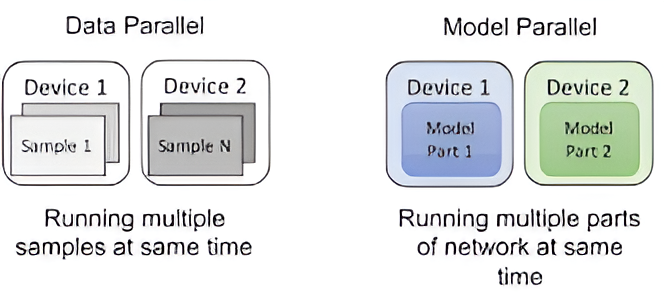
\includegraphics[width=\textwidth]{figures/dml/parallelism_1_1716025674884.png}
        \caption{Parallelism logic depiction}
        \label{fig:parallelism_method}
    \end{subfigure}
    \hfill
    \begin{subfigure}[b]{0.45\textwidth}
        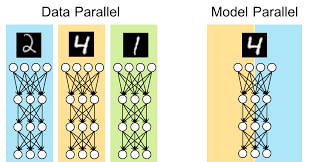
\includegraphics[width=\textwidth]{figures/dml/parallelism.png}
        \caption{An example of model and data parallelism}
        \label{fig:parallelism_example}
    \end{subfigure}
    \caption{Data and Model Parallelism Methods}
    \label{fig:parallelism}
\end{figure}

%%%%%%%%%%%%%%%%%%%%%%%%%%%%%%%%%%%%%%%%%%%%%%%%%%%%%%%%%%%%%%%%%%%%%%%%%%%%%%%
\subsubsection{Distributed Systems Communication Topologies}\label{sec:dml_topologies}
In DML, the communication architecture delineates the specific roles of training nodes. These roles include computation nodes, which compute gradients,
and parameter aggregation nodes, responsible for aggregating these gradients and updating the model parameters. Additionally, it defines the logical
topologies for node communication, such as star or ring configurations. Regardless of the model type and learning objective, the same communication
architecture facilitates parameter exchange and synchronization when using gradient-based optimization algorithms. A Recent article from Liu et al.
~\cite{liuTopologiesDistributedMachine2024} showcases the three primarily used connectivities in Distributed Systems.

\begin{figure}[!ht]
    \centering
    \begin{subfigure}[b]{0.45\textwidth}
        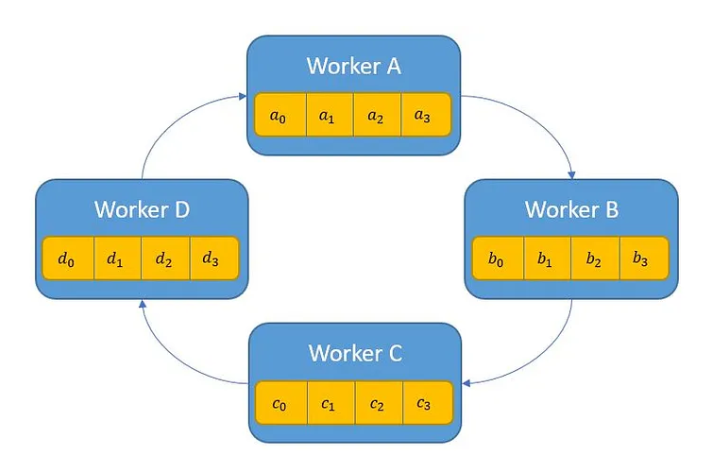
\includegraphics[width=\textwidth]{figures/dml/ring.png}
        \caption{Ring-All Reduce}
        \label{fig:ring}
    \end{subfigure}
    \hfill
    \begin{subfigure}[b]{0.45\textwidth}
        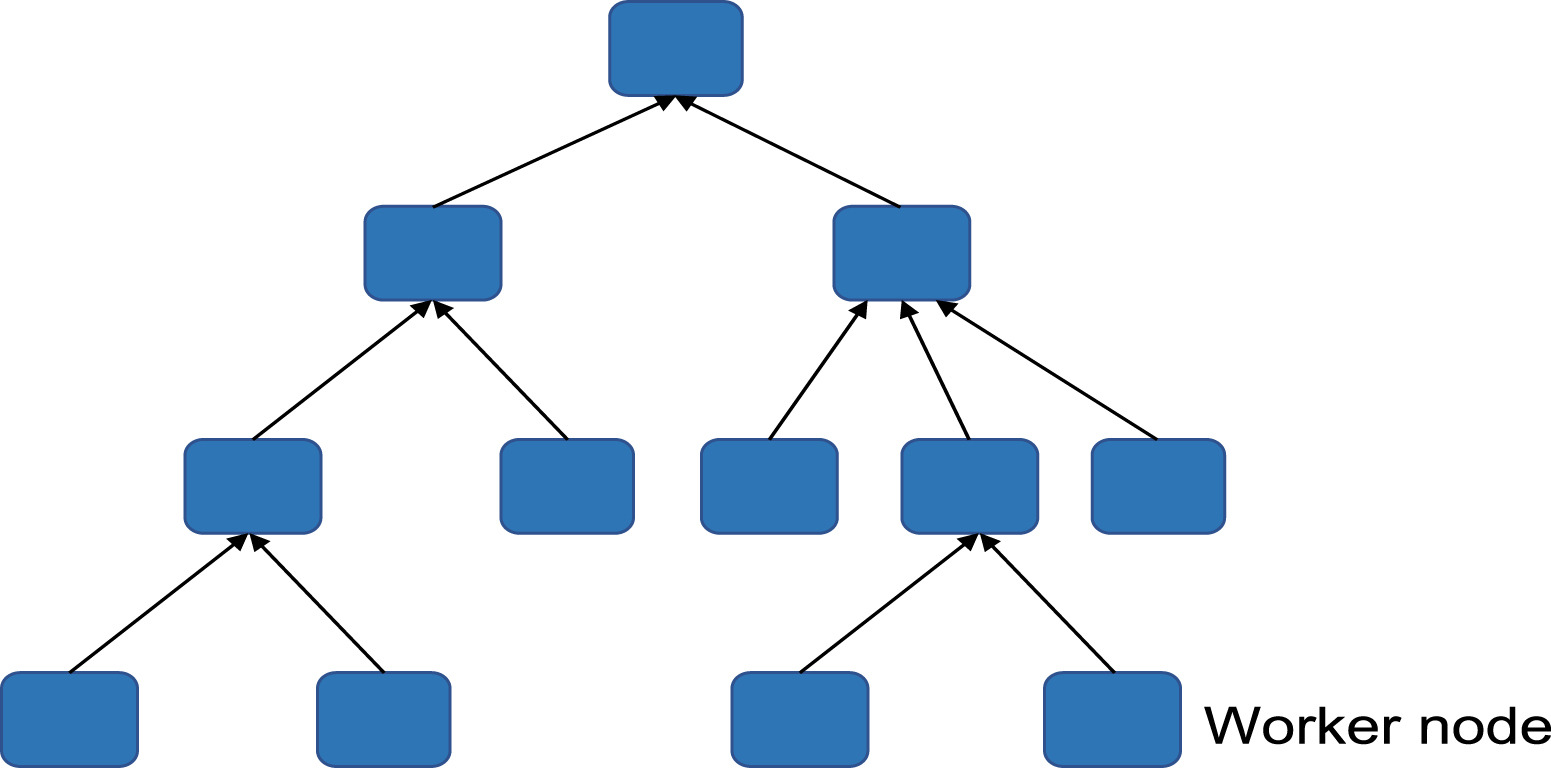
\includegraphics[width=\textwidth, height=0.6\textwidth]{figures/dml/tree.jpg}
        \caption{Hierarchical-Tree}
        \label{fig:tree}
    \end{subfigure}
    \begin{subfigure}[b]{0.6\textwidth}
        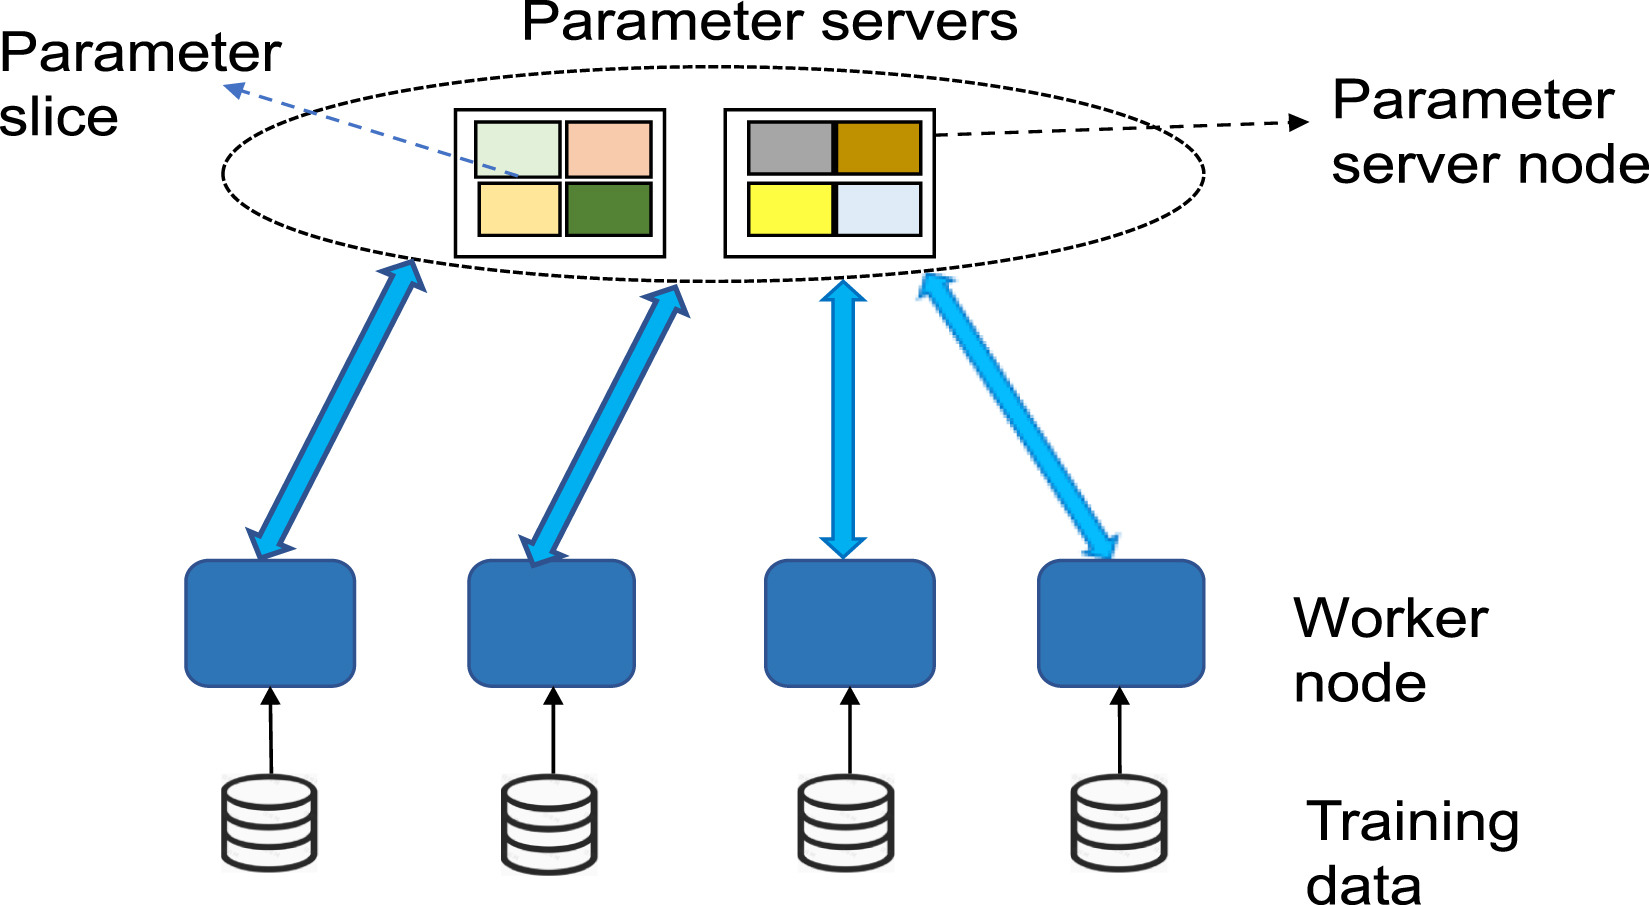
\includegraphics[width=\textwidth]{figures/dml/parameter_server_1.jpg}
        \caption{Decentralized-Parameter Server}
        \label{fig:parameter_server}
    \end{subfigure}
    \caption{Principle Distributed Systems Communication Topologies}
    \label{fig:topologies}
\end{figure}

\begin{itemize}
    \item \emph{Ring-All Reduce:} The Ring architecture arranges nodes in a ring topology, where each node communicates directly with its two neighbors.
          Gradients are shared in a circular manner, with each node sending and receiving data from its adjacent nodes. This architecture efficiently
          utilizes bandwidth by limiting communication to neighboring nodes and avoids the bottlenecks of a centralized coordinator. It is particularly effective
          in GPU clusters and is widely used in distributed deep learning frameworks. A notable example of this topology is the Ring-All Reduce
          implementation provided by Uber's Horovod framework\cite{sergeevHorovodFastEasy2018}.
    \item \emph{Hierarchical-Tree:} The Hierarchical-Tree architecture organizes nodes in a tree structure, where intermediate nodes aggregate gradients
          from their child nodes and pass the aggregated results up the tree to the root node. This reduces the communication overhead compared to a fully
          connected topology and scales efficiently with the number of nodes. The root node eventually computes the global model update and propagates it back
          down the tree. This architecture provides a balance between scalability and communication efficiency\cite{ReillyNetworkDistributed}.
    \item \emph{Decentralized-Parameter Server:} The Decentralized-Parameter Server architecture involves multiple parameter servers distributing the
          management of model parameters. Each worker node communicates with one or more parameter servers to read and update parameters during training. This
          decentralization reduces mitigates bottlenecks and improves fault tolerance compared to a single centralized server. The architecture requires synchronization
          between parameter servers to ensure model consistency across the network.

          This connectivity architecture resembles most the research's implementation,
          yet is restricted to a singular server to mitigate cross-server communication challenges\footnote{Parameter server implementation with a singular server
              resembles a star architecture-all worker nodes directly connected to server}.
          In this scenario, all worker nodes directly communicate with the central server, simplifying network management and reducing latency in communication
          by having a single aggregation point. However, this also introduces a potential bottleneck at the central server and may suffer from single points of failure.
\end{itemize}

%%%%%%%%%%%%%%%%%%%%%%%%%%%%%%%%%%%%%%%%%%%%%%%%%%%%%%%%%%%%%%%%%%%%%%%%%%%%%%%
\subsubsection{Distributed Learning Algorithms}
Last but not least, The DML algorithm selection determines how the learning is conducted after \textit{parallelism method} and \textit{communication topology} are
established. The objective in DML algorithms always remains to leverage parallelism and efficient communication to accelerate training and enable the handling of
large datasets and models that are infeasible for single-machine setups. Therefore, to achieve their goal, data and computation loads are distributed across several
nodes-either being various accelerating devices like GPUs or TPUs or completely different machines\cite{teerapittayanonDistributedDeepNeural2017}.
An outline of an algorithm to achieve the above is presented:

\begin{enumerate}
    \item \emph{Data Preparation:} Partitioning the dataset into subsets that can be distributed across multiple worker nodes,
          ensuring that data distribution maintains the independent and identical distribution (i.i.d.) property when required.
    \item \emph{Model Initialization:} All local models are initialized either locally by each node or centrally by a server and distributed.
          Depending on the needs, the parameters initialization can be random or with a specific model state.
    \item \emph{Local Training:} Each worker node processes its assigned data subset to compute local gradients.
          Parallelism techniques (data parallelism or model parallelism, see \cref{sec:parallelism}) are applied to enhance computational efficiency.
    \item \emph{Gradient Aggregation \& Synchronization:}Gradients computed by each worker are sent either to a server or a peer for aggregation, depending on the topology,
          to update the global model (see \cref{sec:dml_topologies}). Synchronization can be synchronous or asynchronous, affecting the overall training dynamics.
    \item \emph{Model Update:} The updated global model is transmitted back to the worker nodes to reinstate the global
          parameter values to the local model.
    \item \emph{Iteration:} Steps 3 to 5 are repeated until the stopping condition is met.
\end{enumerate}

At this point, we should delve a little deeper into the \emph{Gradient Aggregation \& Synchronization} part outlined previously, in order to sufficiently cover the
principal matter of Synchronization in DML Systems. To be specific, Synchronization can be achieved either in Synchronous or Asynchronous manner in DML systems.
Each of these approaches inevitably comes with some merits and some challenges. In an effort to highlight those, the fundamental optimization algorithms for
gradient calculation, both in Synchronous and Asynchronous Synchronization-namely Synchronous SGD (SSGD) and Asynchronous SGD (ASGD), will be briefly demonstrated.

\paragraph{Synchronous SGD (SSGD)} In SSGD all worker nodes must complete their gradient computations and communicate these gradients before the global model parameters are updated.
This ensures consistency across model updates, as all nodes work with the same model parameters in each iteration. However, this approach can lead to inefficiencies due
to idle times when faster nodes wait for slower ones, also known as the straggler effect. This can impact scalability, especially in large distributed systems where node
performance can vary significantly. On final analysis, the rule to update the parameters, executed by the server at each iteration, can be summarized
~\cite{chenRevisitingDistributedSynchronous2017}:

\begin{equation}
    \label{eq:ssgd}
    w_{t+1} = w_t - \eta \cdot \frac{1}{K} \sum_{i=1}^{K} \nabla f_{\gamma_{t,i}}(w_t)
\end{equation}

Where in the rule above, \emph{$\eta$} denotes the learning rate, \emph{$K$} the number of workers, and \emph{$\gamma_{t,i}$} an index chosen uniformly
at random by the $i$-th worker from ${1,\dots,n}$, representing a selected data point\footnote{It is common in literature to present the SGD approach
    of the algorithm interchangeably with the Mini-Batch approach. This convention is also followed for this research's implementation, so clarification
    was necessary to avoid confusion.}. Thus,  \emph{$\nabla f_{\gamma_{t,i}}(w_t)$} is the stochastic
gradient estimate from the $i$-th worker for the \emph{$\gamma_{t,i}$} data point (or batch).

\paragraph{Asynchronous SGD (ASGD)}
ASGD, conversely, allows worker nodes to proceed with their computations and update model parameters independently of other nodes. This reduces
idle times and can lead to better utilization of computational resources, thereby enhancing scalability. However, the lack of synchronization can result in inconsistencies,
as updates may be based on stale gradients, potentially slowing down the convergence of the model or leading to convergence issues. In Summary, the update rule utilized
in ASSD is\cite{AsynchronousDecentralizedParallel}:

\begin{equation}
    \label{eq:asgd}
    w_{t+1} = w_t - \eta \nabla f_{\gamma_{t,i}}(w_{t - \tau_{i}})
\end{equation}

Where in the rule above, \emph{$\eta$} denotes the learning rate, \(\gamma_{t,i}\) is an index chosen uniformly at random by the \(i\)-th worker
from \(\{1,\dots,n\}\), representing a selected data point, \(\nabla f_{\gamma_{t,i}}(w_{t - \tau_{i}})\) is the stochastic gradient estimate from the
\(i\)-th worker for the \(\gamma_{t,i}\)-th data point, computed at a delayed iteration \( t - \tau_{i} \) due to asynchronous updates.

The choice between Synchronous and Asynchronous SGD is crucial in designing effective DML systems. Synchronous SGD is typically preferred when
consistency and simplicity are paramount, and the computational environment is relatively homogeneous, minimizing the straggler effect.
On the other hand, Asynchronous SGD is advantageous in heterogeneous environments where reducing idle time and improving resource utilization
is critical. The same applies to all the modified and improved variations stemming from these fundamental algorithms that comprise the
cornerstone of DML algorithm implementations.

Conluding, as stated at the beginning of this subsection \cref{sec:dml_architecture} the architecture of a DML system can be decomposed into
the three layers of emph{The Distribution Method (Parallelism)}, \emph{the System's Communication Topology} and \emph{the ML algorithm}. Therefore,
researchers and practitioners of the field need always be aware of the characteristics, both merits and challenges, various designing options
entail, in order to orchestrate efficient and useful DML Systems that can successfully satisfy the problem requirements.

%%%%%%%%%%%%%%%%%%%%%%%%%%%%%%%%%%%%%%%%%%%%%%%%%%%%%%%%%%%%%%%%%%%%%%%%%%%%%%%
%%%%%%%%%%%%%%%%%%%%%%%%%%%%%%%%%%%%%%%%%%%%%%%%%%%%%%%%%%%%%%%%%%%%%%%%%%%%%%%%%%%%%%%%%%%%%%%%%%%%%%%%%%%%%%%%%%%%%%%%%%%%%%%%%%%%%%%%%%%%%%%%%%%%%%%%%%%%%%
\subsection{Challenges in Distributed Machine Learning}
\label{sec:dml_challenges}
Distributed Machine Learning (DML) offers significant advantages in processing large datasets and complex models by leveraging parallelism and
distributed resources. However, it also introduces several challenges, some of which are depicted in \cref{tab:dml_challenges}, that can impact efficiency,
scalability, consistency, and security. These challenges are critical to understand as they set the stage for the transition to Federated
Learning (FL), which addresses several of these issues.

\begin{table}[h!]
    \centering
    \begin{tabular}{>{\raggedright}p{4cm} >{\raggedright}p{7cm} >{\raggedright\arraybackslash}p{3cm}}
        \toprule
        \rowcolor{lightgray}
        \textbf{Challenge}     & \textbf{Description}                                                                                                                                                   & \textbf{Addressed by FL} \\
        \midrule
        Communication Overhead & Frequent communication for gradient updates and synchronization can lead to significant overhead, particularly in environments with limited bandwidth or high latency. & Yes                      \\
        \midrule
        Privacy and Security   & Distributed systems are vulnerable to privacy breaches and security attacks, as data is transferred across nodes and potentially exposed to unauthorized access.       & Yes                      \\
        \midrule
        Data Heterogeneity     & Data distributed across nodes may not be identically and independently distributed (non-IID), leading to biases and inconsistencies in model training.                 & Yes                      \\
        \midrule
        Scalability            & Managing communication and synchronization efficiently becomes challenging as the number of nodes increases, potentially incurring high costs.                         & Partially                \\
        \midrule
        Fault Tolerance        & Ensuring reliability and fault tolerance in a distributed setting is complex, requiring robust mechanisms to handle node failures and network disruptions.             & No                       \\
        \midrule
        Straggler Effect       & In synchronous training, faster nodes must wait for slower ones, leading to idle times and inefficient resource utilization.                                           & No                       \\
        \bottomrule
    \end{tabular}
    \caption{Challenges of Distributed Machine Learning}
    \label{tab:dml_challenges}
\end{table}


\paragraph{Transition to Federated Learning}
Federated Learning (FL) builds on the principles of DML but addresses many of its inherent challenges, particularly those related
to data privacy, communication overhead, and data heterogeneity. To demonstrate, By preserving the training dataset locally Federated Learning
never utilizes the network for private data transmission, negating that way any ill-advised privacy infringements. Moreover, By enabling
local training on edge devices and aggregating only the necessary updates at the end of a learning round, FL restricts network utilization
and additionally enhances privacy. It should be noted also, that Federated Learning systems do not function under the assumption of i.i.d.
data which frequently cannot be stated for other DML system setups. Finally, scalability is partially enhanced due to the overall resetriction
of communication overheads, as only model update transmission are executed and no data transfers leading to more system resources being available,
then again, this performance improvement cannot be objectively measured and in some cases is negligible.

This transition from DML to FL represents an evolution towards more efficient, scalable,
and secure machine learning practices, leveraging distributed resources while mitigating the traditional challenges of DML systems.
In summary, the challenges of DML portrayed at \cref{tab:dml_challenges} highlight the need for more advanced approaches like
Federated Learning. FL addresses these issues by enabling decentralized data processing and focusing on privacy-preserving methods,
making it a crucial advancement for modern machine learning applications, as will be further illustrated in the next section.

%%%%%%%%%%%%%%%%%%%%%%%%%%%%%%%%%%%%%%%%%%%%%%%%%%%%%%%%%%%%%%%%%%%%%%%%%%%%%%%
%5
\section{Federated Learning}
In an era where cloud computing is the dominant paradigm for learning, Federated Learning (FL) has the potential to
drive significant future changes in the industry. Despite the cloud computing market being dominated by
tech giants like Google, Amazon, and Microsoft, Google was the first to recognize the emerging need for a
democratized approach to machine learning. Taking a leading role in Federated Learning research, Google
introduced the term in 2016 with a seminal paper on efficient Distributed Learning\cite{mcmahanCommunicationEfficientLearningDeep2023b}.
The significance of Google’s approach cannot be overstated, as it eliminates the need for maintaining
centralized data centers, allowing cloud resources to be allocated for various other purposes.

% \begin{figure}[!ht]
%     \centering
%     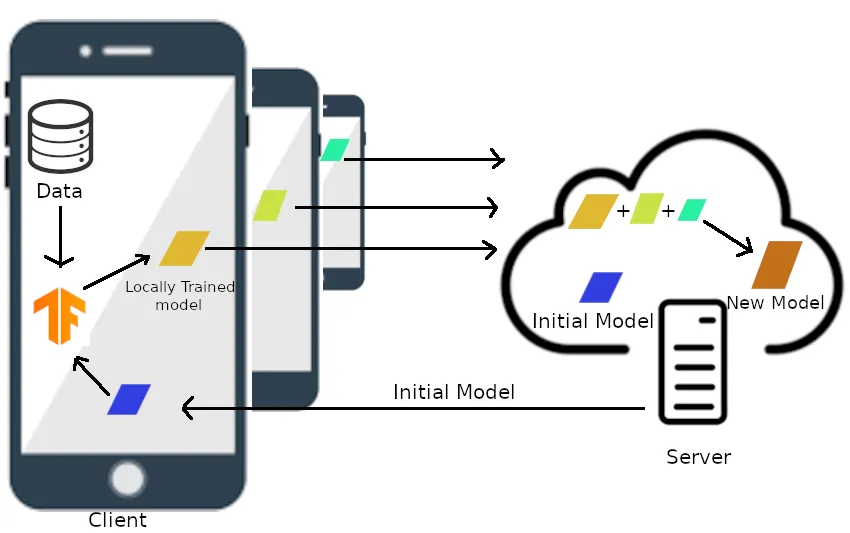
\includegraphics[width=.6\textwidth]{figures/fl/fl.png}
%     \caption{Federated Learning Illustration.}
%     \label{fig:label}
% \end{figure}

The term FL represents a significant shift in how machine learning models are trained and how
data privacy is preserved. As an advanced paradigm within Distributed Machine Learning (DML), FL enables
the training of models across multiple decentralized devices or servers holding local data samples, without
the need to transfer data to a central server. This approach addresses several critical challenges inherent
in traditional centralized machine learning, including data privacy, communication overheads, and the
handling of heterogeneous data and systems.

\begin{figure}[!ht]
    \centering
    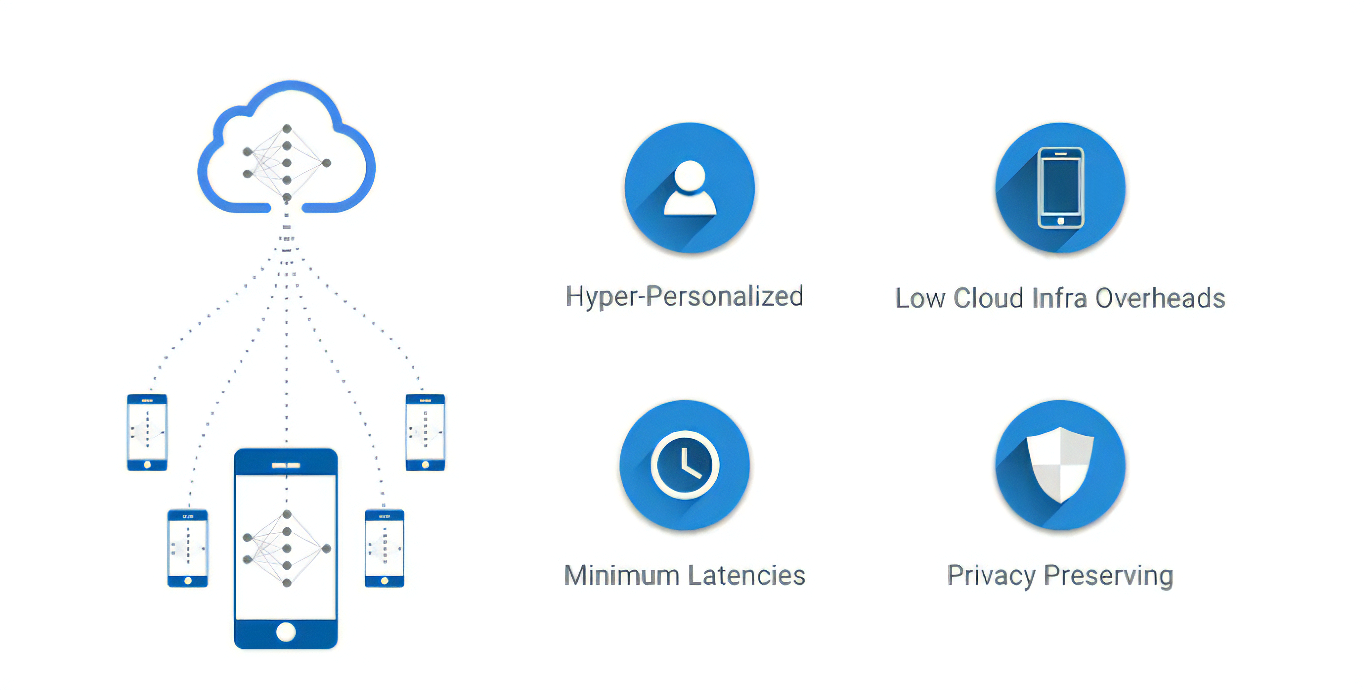
\includegraphics[width=.9\textwidth]{figures/fl/fl_advantages.png}
    \caption{Federated Learning Characteristics.}
    \label{fig:fl_characteristics}
\end{figure}

\subsection{Principles of Federated Learning}
Providing a solution to these issues FL emerged by enabling model training across decentralized devices or
servers while keeping the data local. This method is particularly relevant in scenarios where data privacy is
paramount, such as healthcare, finance, and personal devices like smartphones. A variety of FL applications can
be located in everyday examples-namely image and video automatic categorization, personalized feeds of news
or advertisements, and autocorrect and predictive text (f.i. Google's GBoard\cite{xuFederatedLearningGboard2023}).

\noindent The fundamental principles that determine FL's functionality are categorized as follows\cite{hacksFederatedLearningParadigm2024}:
\begin{itemize}
    \item \emph{Local Data Stays Local:} Data generated by devices or organizations remains on the local device, preventing
          the exposure of sensitive information to external threats or privacy breaches, as it does not need to be uploaded
          to a centralized server for processing.
    \item \emph{Collaborative Model Training:} A central server distributes a global model to devices, which update it based
          on their local data. These updates, typically in the form of gradients or parameters, are sent back to the server and aggregated
          to enhance the global model iteratively, thus improving accuracy and utility without accessing the raw data.
    \item \emph{Privacy by Design:} FL integrates privacy-preserving mechanisms such as secure multi-party computation and
          differential privacy, ensuring that model updates shared with the server do not disclose sensitive information
          about the underlying data or individuals. The privacy rules that are applied, are determined both by international organisms\footnote{Privacy
              preserving legislations such as the General Data Protection Regulation (GDPR) in the European Union
              and the California Consumer Privacy Act (CCPA) in the United States\cite{GeneralDataProtection,CaliforniaConsumerPrivacy}.}
          and local authorities relevant to the region.
    \item \emph{Efficiency and Scalability:} By processing data locally and exchanging only small model updates, FL reduces bandwidth
          requirements for model training, making it scalable across numerous devices and participants, each contributing
          to the refinement of the global model.
\end{itemize}


%%%%%%%%%%%%%%%%%%%%%%%%%%%%%%%%%%%%%%%%%%%%%%%%%%%%%%%%%%%%%%%%%%%%%%%%%%%%%%%%%%%%%%%%%%%%%%%%%%%%%%%%%%%%%%%%%%%%%%%%%%%%%%%%%%%%%%%%%%%%%%%%%%%%%%%%%%%%%%
\subsection{Federated Learning Categorizations}
Several criteria can be used to determine a holistic categorization of Federated Learning (FL) approaches\cite{caruccioSurveyingFederatedLearning2024}.
For the purpose of this research study, the two principal factors are the scale of learning and the alignment of the distributed data. Based on
the learning scale, the separation is executed into Cross-Device and Cross-Silo settings. Based on the data distribution, the
categorization is between Horizontal and Vertical learning settings. The terms presented above will be explained next:

\paragraph{Nature of the Participants:} The distinction is based on whether the federated learning system involves numerous personal
or edge devices (cross-device) or a smaller number of institutions or organizations (cross-silo).

\paragraph{Alignment of the Distributed Data:} The distinction is based on whether the datasets across entities share the same feature
space but have different samples (horizontal) or share the same sample space but have different features (vertical).

%%%%%%%%%%%%%%%%%%%%%%%%%%%%%%%%%%%%%%%%%%%%%%%%%%%%%%%%%%%%%%%%%%%%%%%%%%%%%%%

\begin{figure}[!ht]
    \centering
    \begin{subfigure}[b]{0.45\textwidth}
        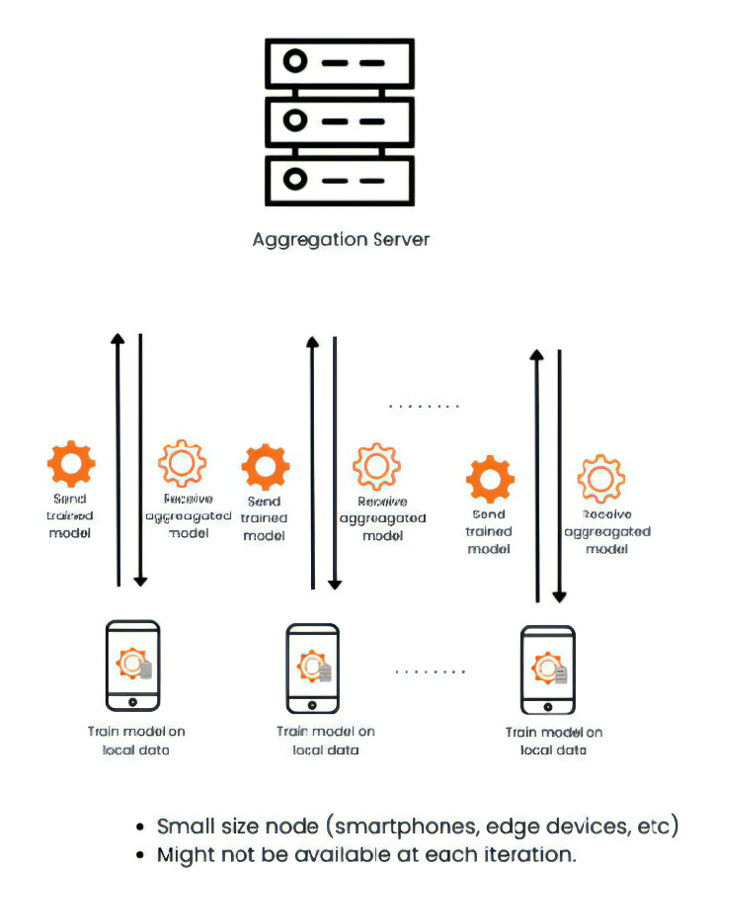
\includegraphics[width=\textwidth]{figures/fl/devices.png}
        \caption{Cross-Device Learning.}
        \label{fig:device}
    \end{subfigure}
    \hfill
    \begin{subfigure}[b]{0.45\textwidth}
        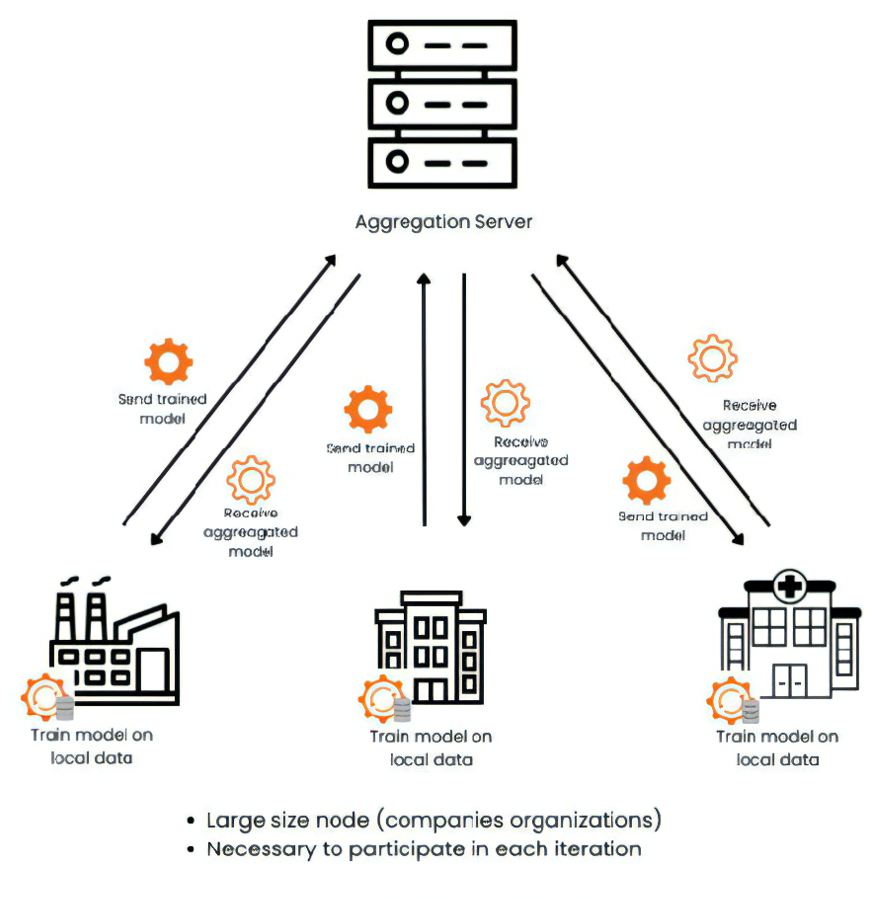
\includegraphics[width=\textwidth, height=1.15\textwidth]{figures/fl/silos.png}
        \caption{Cross-Silo Learning.}
        \label{fig:silo}
    \end{subfigure}
    \caption{Federated Systems separation in Cross-Device or Cross-Silo scale}
    \label{fig:fl_cat_scale}
\end{figure}

\paragraph{Cross-Device Federated Learning}
Cross-device FL involves training models on a large number of edge devices such as smartphones and IoT devices (see \cref{fig:device}). Each device
holds a small, local dataset. This type of FL is particularly useful for applications where individual user data is sensitive,
and thus cannot be shared directly. The primary challenges include managing the diversity in device capabilities, ensuring
efficient communication, and maintaining data privacy. Techniques like asynchronous updates and efficient gradient compression
are often employed to address these challenges\cite{mcmahanCommunicationEfficientLearningDeep2023,chenDistributedLearningWireless2021}
%%%%%%%%%%%%%%%%%%%%%%%%%%%%%%%%%%%%%%%%%%%%%%%%%%%%%%%%%%%%%%%%%%%%%%%%%%%%%%%
\paragraph{Cross-Silo Federated Learning}
Cross-silo FL is used when a small number of organizations, such as hospitals or financial institutions, collaborate to
train a machine learning model (see \cref{fig:silo}). Each organization (silo) has a larger dataset, but data cannot be shared due to privacy concerns.
This method often aligns with regulatory requirements such as GDPR and CCPA\@. Challenges include managing non-IID data distributions
across silos and ensuring secure aggregation of model updates. Techniques like secure multi-party computation (SMPC) and differential
privacy are crucial in this context\cite{yangFederatedMachineLearning2019,zhaoFederatedLearningNonIID2018}.


%%%%%%%%%%%%%%%%%%%%%%%%%%%%%%%%%%%%%%%%%%%%%%%%%%%%%%%%%%%%%%%%%%%%%%%%%%%%%%%
%%%%%%%%%%%%%%%%%%%%%%%%%%%%%%%%%%%%%%%%%%%%%%%%%%%%%%%%%%%%%%%%%%%%%%%%%%%%%%%%%%%%%%%%%%%%%%%%%%%%%%%%%%%%%%%%%%%%%%%%%%%%%%%%%%%%%%%%%%%%%%%%%%%%%%%%%%%%%%
\subsubsection{Horizontal and Vertical Federated Learning}

\paragraph{Horizontal Federated Learning (HFL)}
HFL, or sample-based FL, occurs when different entities (devices or institutions) have datasets with the same feature space
but different samples. For instance, multiple hospitals might have patient records with the same attributes. HFL is commonly
used in both cross-device and cross-silo settings. The main challenge is handling non-IID data, where each client’s data
distribution may vary significantly. Approaches like data augmentation and federated averaging (FedAvg) are often used to
mitigate these issues\cite{konecnyFederatedOptimizationDistributed2016}.

%%%%%%%%%%%%%%%%%%%%%%%%%%%%%%%%%%%%%%%%%%%%%%%%%%%%%%%%%%%%%%%%%%%%%%%%%%%%%%%
\paragraph{Vertical Federated Learning (VFL)}
VFL, or feature-based FL, occurs when entities have datasets with different feature spaces but the same sample space. For
example, one organization might have transaction data, while another has demographic data about the same customers. VFL is
typically used in cross-silo settings. The primary challenge is ensuring secure and efficient computation when combining
different types of data. Secure computation techniques and feature alignment methods are critical to address these challenges
~\cite{yangFederatedMachineLearning2019,chenDistributedLearningWireless2021}.

\begin{figure}[!ht]
    \centering
    \begin{subfigure}[b]{0.45\textwidth}
        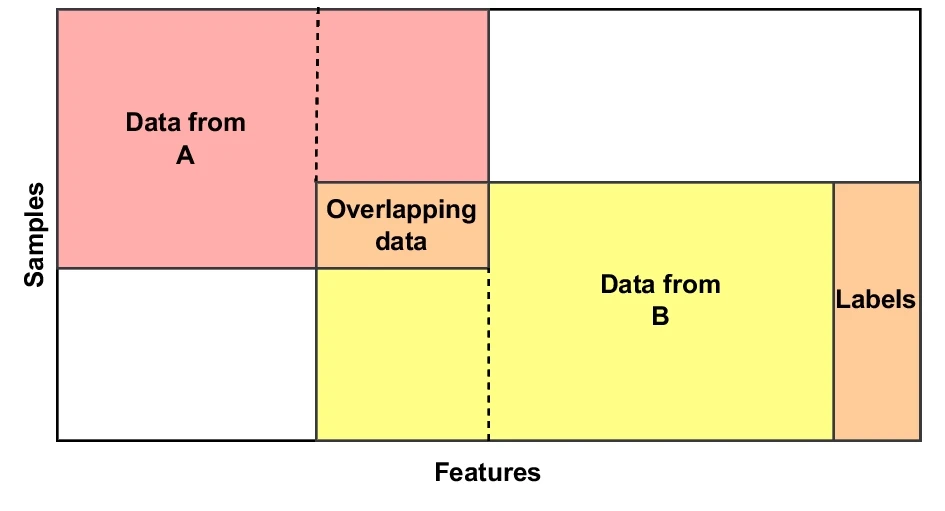
\includegraphics[width=\textwidth]{figures/fl/horizontal.png}
        \caption{Horizontal Federated Learning.}
        \label{fig:horizontal}
    \end{subfigure}
    \hfill
    \begin{subfigure}[b]{0.45\textwidth}
        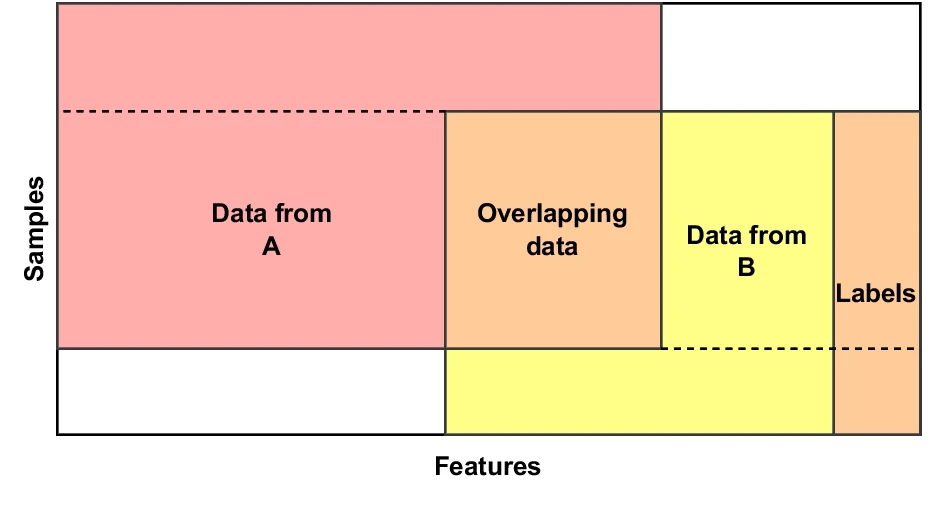
\includegraphics[width=\textwidth]{figures/fl/vertical.png}
        \caption{Vertical Federated Learning.}
        \label{fig:vertical}
    \end{subfigure}
    \caption{Federated Systems separation in horizontal or vertical learning\cite{caruccioSurveyingFederatedLearning2024}.}
    \label{fig:fl_cat_distribution}
\end{figure}
%%%%%%%%%%%%%%%%%%%%%%%%%%%%%%%%%%%%%%%%%%%%%%%%%%%%%%%%%%%%%%%%%%%%%%%%%%%%%%%
%%%%%%%%%%%%%%%%%%%%%%%%%%%%%%%%%%%%%%%%%%%%%%%%%%%%%%%%%%%%%%%%%%%%%%%%%%%%%%%%%%%%%%%%%%%%%%%%%%%%%%%%%%%%%%%%%%%%%%%%%%%%%%%%%%%%%%%%%%%%%%%%%%%%%%%%%%%%%%
\subsection{Federated Learning Methodology}
\subsubsection{Architecture}
In a Federated Learning setup, the architecture can be decomposed into four principal parts:
The client devices, the central server, the communication protocols, and the security mechanisms.
An overview of each component's functionality will be presented for a typical Federated Learning Architecture
based on the cumulative analysis provided by multiple
literature sources\cite{mcmahanCommunicationEfficientLearningDeep2023,yangFederatedMachineLearning2019,
    konecnyFederatedOptimizationDistributed2016,bhoseDifferentiatingDistributedLearning2023}.
It is avoided to delve further into details for some of the presented terms in cases where they are not
relevant to the research's objectives. In those circumstances, just a conceptual illustration is provided.

\paragraph{Client Devices:} Client devices are the edge devices or local servers that generate and hold the local data.
These can include smartphones, IoT devices, or organizational databases. Each client device performs local training on
its dataset, updating the model’s parameters based on local data. This helps preserve data privacy since the raw data
never leaves the device. After training locally, the clients send their model updates (e.g., gradients or parameters)
to the central server. These updates are computed using the local data, ensuring that sensitive or personal information
is not exposed. The heterogeneity of these devices, in terms of computational power and network connectivity, presents
a challenge that must be managed by the system.

\paragraph{Central Server:} The central server acts as a coordinator that aggregates model updates from multiple
client devices and updates the global model. Essentially, the server collects model updates sent by the clients, aggregates
these updates to refine the global model, and then redistributes the updated global model back to the clients for further
training iterations. This process ensures that the global model improves iteratively based on the decentralized data from
all participating clients. The central server must handle the challenges of aggregating updates efficiently and securely
to maintain the model's performance and integrity.

\paragraph{Communication Protocols:}\label{par:communication} The communication protocol defines the rules and methods for data exchange between
client devices and the central server. Efficient communication protocols are essential to minimize latency and bandwidth
usage during the model update exchanges. Protocols in FL often incorporate techniques to reduce the volume of data transferred,
such as model compression and gradient sparsification. Asynchronous communication methods can handle the varying availability and
performance of client devices, reducing overall training time and mitigating the straggler effect.

\paragraph{Security Mechanisms:}\label{par:security} Security mechanisms are critical in FL to ensure that the data and model updates remain confidential and tamper-proof.
These mechanisms protect against potential attacks that could compromise the privacy and integrity of the data being processed.
Common security measures include encryption, differential privacy, and secure multi-party computation (SMPC). Encryption ensures that data
transmitted between clients and the server is protected from eavesdropping. Differential privacy adds noise to the model updates to prevent the
reconstruction of sensitive data. SMPC allows multiple parties to compute a function over their inputs while keeping those inputs private, further
enhancing the security of the federated learning process.

%%%%%%%%%%%%%%%%%%%%%%%%%%%%%%%%%%%%%%%%%%%%%%%%%%%%%%%%%%%%%%%%%%%%%%%%%%%%%%%%%%%%%%%%%%%%%%%%%%%%%%%%%%%%%%%%%%%%%%%%%%%%%%%%%%%%%%%%%%%%%%%%%%%%%%%%%%%%%%
\subsection{Problem Formulation in Federated Learning}
This section provides a clear a clear overview of the FL problem statement based on the Almanifi et al.\ article (2023)\cite{almanifiCommunicationComputationEfficiency2023}
observations.
In the broader field of Machine Learning (ML), the primary problem is to learn a model that maps a set of input data \( x \) to a set of
desired outputs \( y \) based on a number of training examples. The performance of this model is evaluated using a loss function \( f_i(w) \),
which measures the error between the model's predictions and the actual desired outputs. For a set of \( n \) input-output pairs $\{x_i, y_i\}_{i=1}^n$,
the goal is to find the optimal weight vector(s) \( w \) that minimizes the loss function. An example of this in a linear regression problem is:

\begin{equation}
    f_i(w) = \frac{1}{2}(x_i^T w - y_i)^2, \quad y_i \in \mathbb{R} \text{ and } x_i \in \mathbb{R}^d
\end{equation}

Although loss functions vary across different ML techniques, the problem generally can be formulated as an optimization problem for a
finite-sum of functions, expressed as:

\begin{equation}
    \label{eq:objctive_func_fedAVG}
    \min_{w \in \mathbb{R}^d} f(w) \quad \text{where} \quad f(w) = \frac{1}{n} \sum_{i=1}^n f_i(w)
\end{equation}

In Federated Learning, the training process minimizes the loss function locally through gradient descent before the
weights \( w \) are communicated to the central server. Consider an FL system
with a fixed number of clients \( K \), where each client hosts a partition of the data \( n_k \), indexed by
\( \mathcal{P}_k = \{1, 2, \ldots, i\} \). Upon receiving all local parameters, the global server aggregates \( w \) to update the
new global model. The aggregation mechanism sets the global objective. For example, in FedAVG, one of the most commonly used aggregation
methods in FL, the loss function is updated to:

\begin{equation}
    f(w) = \sum_{k=1}^K \frac{n_k}{n} F_k(w) \quad \text{where} \quad F_k(w) = \frac{1}{n_k} \sum_{i \in \mathcal{P}_k} f_i(w)
\end{equation}

Thus, the problem in FL becomes learning the aforementioned model in a distributed manner without exchanging raw data.

%%%%%%%%%%%%%%%%%%%%%%%%%%%%%%%%%%%%%%%%%%%%%%%%%%%%%%%%%%%%%%%%%%%%%%%%%%%%%%%%%%%%%%%%%%%%%%%%%%%%%%%%%%%%%%%%%%%%%%%%%%%%%%%%%%%%%%%%%%%%%%%%%%%%%%%%%%%%%%
\subsubsection{Federated Learning Process} \label{sec:fed_learning_process}
\begin{figure}[!ht]
    \centering
    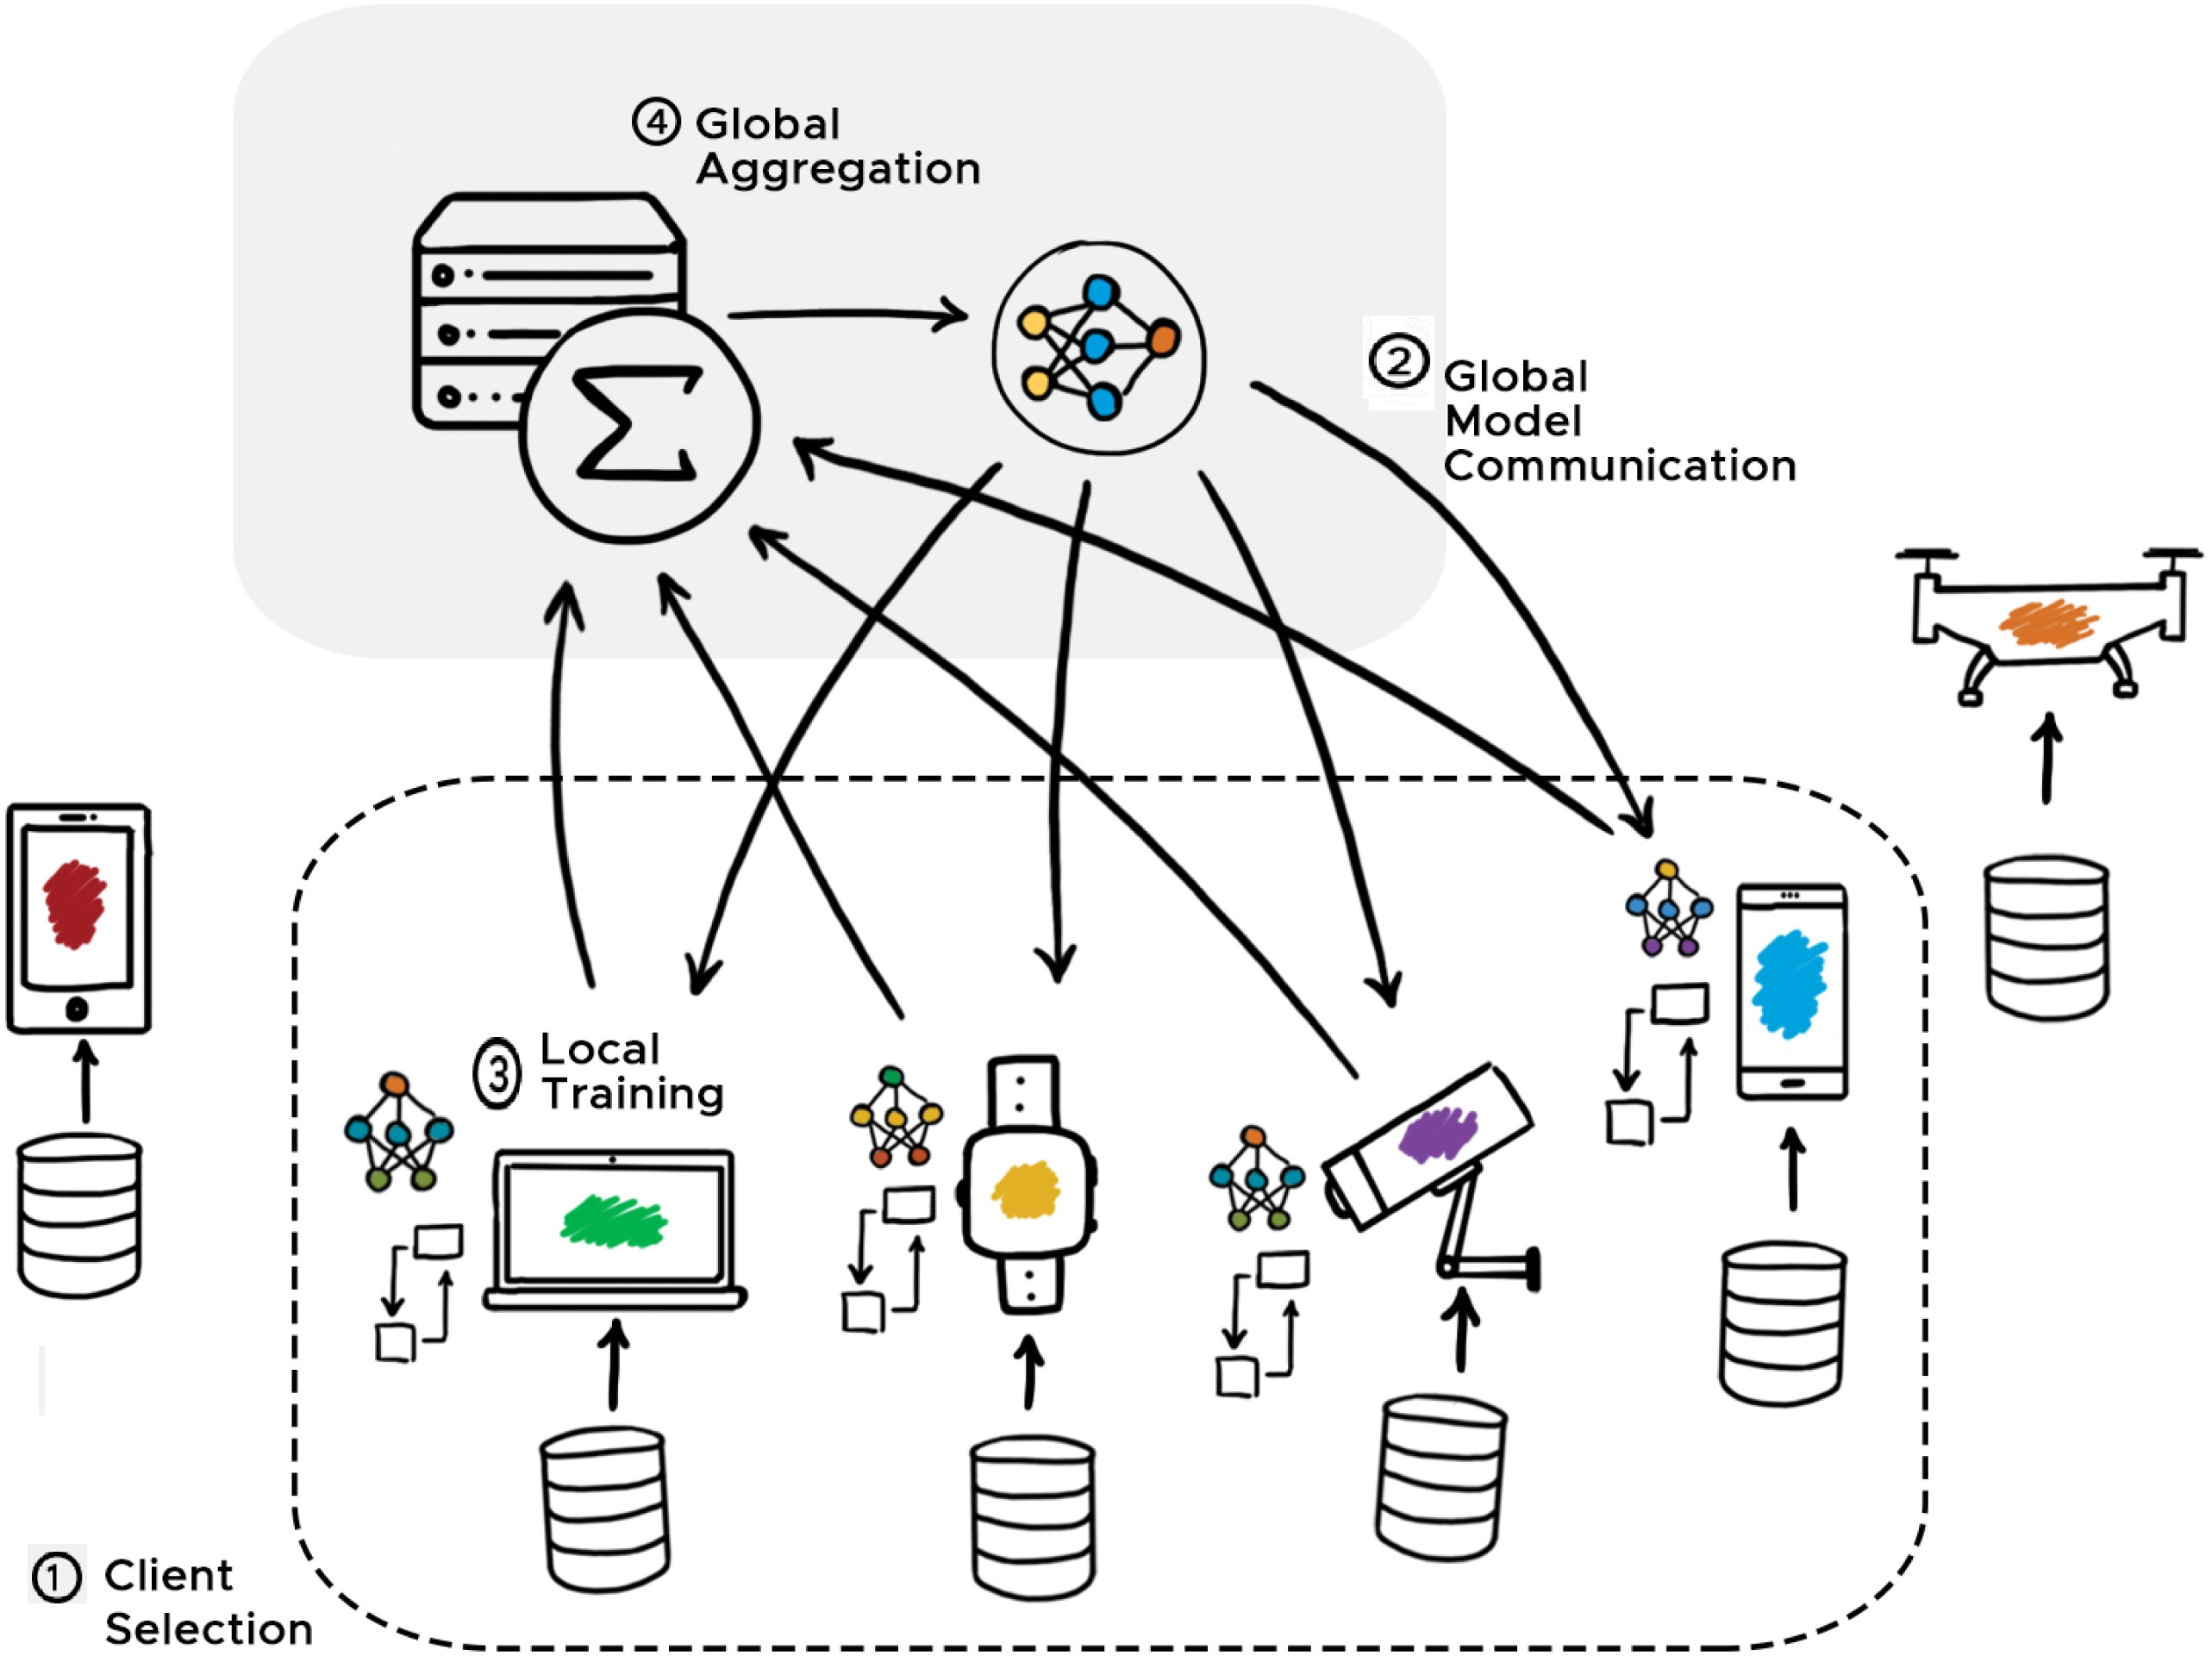
\includegraphics[width=.8\textwidth]{figures/fl/fl_2.jpg}
    \caption{General FL training process\cite{almanifiCommunicationComputationEfficiency2023}.}
    \label{fig:fl_process}
\end{figure}

In distributed machine learning setups, such as Federated Learning, processes are often viewed as continuous, meaning that the system continuously
updates and refines the model parameters based on incoming data. This continuous process allows for dynamic adjustments and real-time improvements,
making the system more adaptive and responsive to changes in the data\cite{deanLargeScaleDistributed2012,almanifiCommunicationComputationEfficiency2023}.
Provided that, in the iterative training process, each iteration/round can be separated into four major steps as displayed in \cref{fig:fl_process}:

\begin{enumerate}

    \item \emph{Client Selection:} Selection strategies vary, as client selection can be executed either randomly, or with prioritization criteria in mind.
          Depending the FL setup, client selection can be conducted at two different stages: either before sending the global model
          to the clients (first step) or after local training (third step).
          \emph{First Step Selection}: The central manager selects a subset of clients before sending the global model. This pre-selection
          can be used to restrict the number of clients that participate in training, while also gives the opportunity to filter clients based
          on their update quality.
          \emph{Third Step Selection}: After local training, the server selects a subset of clients to transmit their model updates. This step
          prevents diminishing returns seen when the full set of clients is used.  In our implementation client selection is conducted before the
          global model communication.

    \item \emph{Global Model Communication:} The process begins with available clients notifying the server of their readiness to participate. The server then
          communicates the global model to all participating clients, signaling the beginning of the communication round. This step involves broadcasting the global
          model's parameters, which include weights and biases, along with any relevant metadata such as hyperparameters (e.g., learning rate) and other arguments
          (e.g., batch size).

    \item \emph{Local Training:} Each client trains the model locally using its own local dataset. During this step, the clients adjust the global model
          parameters based on their local data, resulting in a \emph{Model Update}. The training process is conducted according to the instructions and
          hyperparameters provided by the server. The objective function of the training process is notated as \( f \), and for a selected client \( n \)
          from the set of clients \( N \), it attempts to minimize its loss function \( L \), which depends on the global model weights \( w_g \) and the
          local data \( d_i \):

          \begin{equation}
              f_n(w_g) = \arg\min_{n \in N} L(w_g; d_n)
          \end{equation}
          After training, clients need to transmit their model updates back to the central server for aggregation (see \cref{en:aggregation}).
          The model updates may undergo additional processing to enhance efficiency and security, as outlined in \cref{par:communication}.
          Finally, the processed model updates are transmitted to the server, and the clients remain inactive until selected again.

    \item \emph{Global Aggregation:}\label{en:aggregation}
          Upon receiving the updated parameters from each selected client, the server aggregates them into a global model using a chosen aggregation
          mechanism. Various strategies can be employed, such as the FedAVG method, which averages the updates from the clients. The global objective
          is to minimize the overall loss function as shown in \cref{eq:objctive_func_fedAVG}. Once the model is updated, the communication round ends.
          The server then evaluates the global model's performance using metrics over a public test set. Based on this evaluation, training may be
          terminated if the desired accuracy is achieved or the preset number of rounds is completed; otherwise, a new communication round begins.
\end{enumerate}

The above functionality describes a synchronous federated learning setup, which aligns with the thesis implementation. However, as highlighted earlier
in order to improve a distributed system's performance, asynchronous methods can be applied too, mitigating the straggler effect.

% While programming an asynchronous learning system is taxing and requires careful considerations about out-of-sync updates, the fundamental logic remains the same.
% Building on the outlined learning procedure above, the only things that would be modified in a asynchronous setup, is the removal of synchronization 
% mechanisms. Specifically, unlike the synchronous counterpart, in asynchronous clients can start and finish training in different times. 

While programming an asynchronous learning system is taxing and requires careful considerations about out-of-sync updates, the fundamental logic remains the same
with modifications primarily pertain to the timing and coordination of these steps. To be exact, In an asynchronous federated learning setup, client selection remains dynamic,
but clients are allowed to start and finish their local training at different times. This flexibility means that the server can receive and aggregate updates from
clients as they become available, without waiting for all selected clients to complete their training. Consequently, global model communication is also more fluid,
with the server sending the global model to clients on an as-needed basis, rather than all at once. Local training on each client still follows the same process,
but clients send their updates to the server independently upon completion. The server continuously aggregates these updates using the chosen aggregation mechanism,
such as weighted averaging, and updates the global model iteratively.



%%%%%%%%%%%%%%%%%%%%%%%%%%%%%%%%%%%%%%%%%%%%%%%%%%%%%%%%%%%%%%%%%%%%%%%%%%%%%%%
%6
\section{Networking in Federated Systems}
\subsection{Network Topologies}
\label{sec:fl_topologies}
The underlying network infrastructure plays a crucial role in the performance and scalability of Federated Learning FL and
Distributed Machine Learning systemsm, in general. Three of the most prevalent topologies employed in DML Systems where described
earlier in \cref{sec:dml_topologies}. Likewise, it can be stated that, by being a subset of DML systems Federated Systems are
constructed using the same fundamental topologies. That said, FL Systems are indeed typically arranged in star, hierarchical
tree, ring or peer-to-peer topologies.

Recapitulating briefly in regards with FL, \emph{star topologies}, are a simplification of parameter server setups, where $N$ clients are directly
connected with one central server (parameter server) who coordinates the learning procedure. The star topology is advantageous for its
simplicity and ease of implementation. However, it can become a bottleneck and a single point of failure, limiting the system's scalability and
robustness.

\emph{Hierarchical tree topologies}, differ from star topologies due to the fact that clients do not always communicate directly with the server.
Instead they might be organized in smaller clusters of $M$ clients where $M < N$, that transmit their model updates to intermediate stations
responsible for aggregating local model updates, communicating the intermediate aggregation results to the server.
This hierarchical approach can improve scalability by distributing the aggregation workload and reducing the communication burden on the central
server. Additionally, it can enhance fault tolerance by localizing the impact of network failures.

\emph{Ring setups} indicate that each node communicates directly with its two neighbors. This way, communication is conducted in a circular manner,
presenting a peer-to-peer approximation approach where the coordination responsibility is distributed to the workers. This topology can provide
robustness and fault tolerance, as the failure of a single node does not disrupt the entire network. However, it may suffer from higher latency
as the number of nodes increases due to the sequential nature of communication.

Finally, In a \emph{fully peer-to-peer} setup, clients communicate directly with each other broadcasting their model udpates without a central coordinting authority.
Protocols such as gossip algorithms are used to propagate updates throughout the network. This approach can enhance privacy and decentralization but may
require more complex coordination mechanisms.

Overall, it becomes obvious that the selection of each of these topologies for the design of a FL system entails certain merits and challeges
in regards with the communication effiecincy.
This fact can be observed directly through network related metrics such as latency, throughput

%%%%%%%%%%%%%%%%%%%%%%%%%%%%%%%%%%%%%%%%%%%%%%%%%%%%%%%%%%%%%%%%%%%%%%%%%%%%%%%%%%%%%%%%%%%%%%%%%%%%%%%%%%%%%%%%%%%%%%%%%%%%%%%%%%%%%%%%%%%%%%%%%%%%%%%%%%%%%%
\subsection{Communication in Federated Systems}
\subsubsection{Communication Protocols}
The communication protocol defines the rules and methods for data exchange between client devices and the
central server. Efficient communication protocols are essential to maximize perfomance during model exchange procedures.
There is a plethora of contempory technologies with diverse characteristics being utilized in Federated communication, with
most primary examples being gRPC, Protocol Buffers (Protobuf), WebSockets, and HTTP/2 and TCP Sockets.

\begin{itemize}
    \item \emph{gRPC} is a high-performance, open-source Remote Procedure Call (RPC) framework that can run in any environment.
          It uses HTTP/2 for transport, Protocol Buffers (protobuf) as the interface description language, and prSovides features such as
          authentication, load balancing, and more. The efficient serialization and transport mechanisms of gRPC make it well-suited for
          federated learning scenarios where low latency and high throughput are crucial.

    \item \emph{HTTP/2} is a major revision of the HTTP network protocol, focusing on performance improvements. It introduces features
          like multiplexing, header compression, and server push. This protocol has become a industry standard due to its unmatched efficiency.

    \item \emph{Protobufs (Protocol Buffers)} are a language-neutral, platform-neutral, extensible mechanism for serializing structured data.
          Protobuf is used to define the structure of the messages-namely model parameters, training configurations, and results exchanged
          between the server and clients. This ensures efficient and compact communication.

    \item \emph{WebSockets} provide a full-duplex communication channel over a single, long-lived TCP connection. They are useful
          for real-time applications requiring continuous data exchange. Thet makes WebSokcets the first choice when maintaining a persistent
          connection between the server and clients is beneficial. This can be particularly useful in real-time monitoring and control of the
          FL process.

    \item \emph{TCP Sockets} offer a reliable, connection-oriented communication protocol that ensures data integrity and delivery.
          TCP handles packet loss, data corruption, and data reordering, making it suitable for scenarios where reliability is paramount.
          In federated learning, TCP sockets can be used to establish robust connections between the server and clients, ensuring that
          critical updates are transmitted accurately and efficiently.

\end{itemize}

\subsubsection{Communication Enhancement}
\label{sec:con_settings}

The performance of federated learning systems is significantly influenced by the type of connectivity used. Different network types offer
distinct advantages and are preferred in various scenarios:
- \emph{Ethernet}: Provides high reliability and consistent bandwidth, making it ideal for environments requiring stable, high-speed
communication, such as data centers and research facilities where large-scale model training occurs.
- \emph{Wi-Fi}: Offers flexibility and mobility, suitable for residential or office settings where devices are not fixed and may move
around. It is preferred in scenarios like smart homes or collaborative workspaces where user devices frequently change locations.
- \emph{Point-to-Point Connections}: Provide direct and reliable communication paths, preferred in specialized settings such as direct
communication between servers in a data center or between two devices in close proximity that require secure and fast data exchange without
intermediate routers.
- \emph{Cellular Networks (4G/5G)}: Useful for mobile and remote applications where devices are dispersed over large geographical areas.
This is ideal for applications like connected vehicles or remote health monitoring systems, where data needs to be collected from widely
distributed sources.

Regardless of the selected communication protocol, and connectivity setting, communication overheads can always be reduced by minimizing
the size of transmitted data. Techniques such as quantization, compression  and efficient encoding can significantly decrease the amount
of data exchanged between clients and the server, thus reducing latency and improving overall system efficiency.

%%%%%%%%%%%%%%%%%%%%%%%%%%%%%%%%%%%%%%%%%%%%%%%%%%%%%%%%%%%%%%%%%%%%%%%%%%%%%%%%%%%%%%%%%%%%%%%%%%%%%%%%%%%%%%%%%%%%%%%%%%%%%%%%%%%%%%%%%%%%%%%%%%%%%%%%%%%%%%
\subsection{Communication Performance Metrics}

In FL systems, evaluating communication performance is paramount to understanding the efficiency and effectiveness of
distributed learning processes. Several critical metrics are used to assess communication performance, each contributing
to a comprehensive analysis of the system's capabilities and limitations.

\textbf{Latency (\(L\))} is a fundamental metric, representing the time interval required for a message to travel
from the source node to the destination node. It is indicative of the system's responsiveness. Mathematically, latency is defined as:
\[
    L = t_r - t_s
\]
where \( t_s \) is the time a message is sent, and \( t_r \) is the time it is received.


\textbf{Bandwidth (\(B\))} measures the maximum rate at which data can be transmitted over a network connection within a specific
time frame, reflecting the network's capacity to handle data transfers. It is given by:
\[
    B = \frac{D}{T}
\]
where \( D \) is the total amount of data that can be transferred, and \( T \) is the theoretical time taken for the transfer.

\textbf{Throughput (\(T\))} is closely related to bandwidth but focuses on the actual rate of successful data transfer over the network,
considering factors such as network congestion and protocol overhead. In other words, the first one calculates the maximum  theoretically achieved
speed of tranfer of the channel, while the second represents the actual calculated value accomplished in an experiment.
It is defined as:
\[
    T = \frac{D_r}{T_r}
\]

where \( D_r \) is the actual amount of data transferred, and \( T \) is the actual time taken for the transfer. T
\textbf{Packet Loss Rate (PLR)} is the percentage of packets lost during transmission, which can significantly impact the performance of FL systems.
It is calculated as:
\[
    PLR = \frac{P_{sent} - P_{received}}{P_{sent}} \times 100\%
\]
where \( P_{sent} \) is the number of packets sent, and \( P_{received} \) is the number of packets received successfully.

% \textbf{Jitter (\(J\))} refers to the variation in time between packets arriving, caused by network congestion, timing drift, or route changes.
% It is crucial for understanding the stability of the communication link, and to measure the straggler effect in DML systems. Jitter is defined as:
% \[
%     J = \frac{1}{N-1} \sum_{i=1}^{N-1} |t_i - t_{avg}|
% \]
% where \( t_i \) is the time interval between the \(i^{th}\) packet and the \((i-1)^{th}\) packet, and \( t_{avg} \) is the average time interval.

Dropout Rate (\(DR\)) is a significant metric in federated learning, indicating the percentage of clients that fail to complete the training
process due to various reasons such as connectivity issues or resource constraints. It is defined as:
\[
    DR = \frac{N_{dropout}}{N_{total}} \times 100\%
\]
where \( N_{dropout} \) is the number of clients that dropped out, and \( N_{total} \) is the total number of clients.

The Computation-Communication Ratio (\(CCR\)) assesses the balance between computational load and communication overhead in federated systems.
It is crucial for optimizing performance and resource allocation. \( CCR \) is defined as:
\[
    CCR = \frac{C}{C + C_{comm}}
\]
where \( C \) is the time spent on computation, and \( C_{comm} \) is the time spent on communication.

Network characteristics such as latency, bandwidth, reliability, and connection type significantly influence the performance of FL systems.
High latency can delay the synchronization of model updates, while limited bandwidth can restrict the amount of data that can be transmitted
n each communication round. Network reliability ensures that updates from clients are consistently received by the server, while the chosen
topology affects the overall communication overhead. For instance, using TCP sockets ensures reliable data transfer with error checking, and
gRPC facilitates efficient remote procedure calls, both of which are critical for maintaining the integrity of the FL process. Model compression
techniques are also employed to reduce the size of the transmitted updates, thereby mitigating the impact of limited bandwidth and high latency.

\subsection{Simulating Real-World Networks}
Network simulators play a pivotal role in federated learning (FL) research by enabling researchers to test and evaluate the performance of FL systems under various network conditions. This capability is significant because setting up FL environments with numerous devices in a controlled laboratory setting is challenging. Simulators such as \textit{NS-3}, \textit{OMNeT++}, and \textit{Mininet} can emulate real-world network environments, offering valuable insights into how different network characteristics influence the training process.

\subsubsection{Mimicking Real-World Network Conditions}

Simulators can accurately replicate several aspects of real-world networks, including:

\begin{itemize}
    \item \emph{Network Congestion:} By simulating varying levels of network traffic, researchers can observe how congestion impacts data transmission and model updates in FL systems.
    \item \emph{Latency Variability:} Simulators can introduce different latency values to examine how delays in communication affect the synchronization and convergence of models.
    \item \emph{Bandwidth Fluctuations:} Emulating changes in available bandwidth helps in understanding the effect on the speed and efficiency of data exchanges between clients and the central server.
    \item \emph{Error Rates:} Introducing different error rates across multiple clients can mimic real-life scenarios where devices have varying communication capabilities and reliability.
    \item \emph{Network Topologies:} Simulators can model different network topologies, such as star, ring, and hierarchical structures, to study their impact on the performance of FL systems.
\end{itemize}

\subsubsection{Measuring Contributions from Simulations}

Through the use of network simulators, researchers can measure several key performance metrics that provide insights into the effectiveness and robustness of FL systems:

\begin{itemize}
    \item \emph{Impact on Model Convergence:} By analyzing how network conditions such as latency and bandwidth influence the speed and accuracy of model convergence, researchers can identify bottlenecks and optimize communication strategies.
    \item \emph{System Robustness:} Simulating scenarios with multiple clients experiencing varying error rates allows for the assessment of the system's robustness and its ability to handle client dropouts or unreliable connections.
    \item \emph{Scalability Analysis:} Researchers can observe how the FL system scales with the number of clients, particularly when clients have different communication capabilities. This helps in understanding the limits and potential optimizations for large-scale deployments.
    \item \emph{Topology Influence:} Evaluating the effect of different network topologies on system performance provides insights into the most efficient structures for specific FL applications.
\end{itemize}

In summary, network simulators are indispensable tools in FL research, enabling the detailed study of various network conditions and their impact on the training process. They help in identifying potential issues and optimizing FL systems to ensure efficient, scalable, and robust performance in real-world deployments.





%%%%%%%%%%%%%%%%%%%%%%%%%%%%%%%%%%%%%%%%%%%%%%%%%%%%%%%%%%%%%%%%%%%%%%%%%%%%%%%
%7
\section{Summary \&\ Transition to Related Work}
% Part about summarining and connecting 
The theoretical background overview provided in this chapter laid the groundwork for highlighting the
principal elements, definitions and contempory challenges relevant to our \emph{Federated Learning} research.
We began by exploring the broader concept of \emph{Machine Learning} exploring the fundamental principles and
objectives of the learning procees, proceeding with \emph{Artificial Neural Networks} and deep learning to
establish a basis for understanding complex model architectures and contemporary learning paradigms.
Then our analysis took a turn towards \emph{Optimization Techniques}, crucial for enhancing the learning efficiency
of sophisticated, multi-parameter model architectures like the ones employed in \emph{Federated Learning} setups.

Subsequently, the discussion focused on \emph{Distributed Learning Systems}, highligting their significance in managing
learning with immense datasets distributed in a multitude of worker nodes, while preserving computation efficiency.
This naturally led to an in-depth analysis of \emph{Federated Learning}, which builds on distributed learning principles
to enhance data privacy and minimize communication overhead by allowing decentralized data processing and model updates.
To conclude, a brief demonstration of \emph{Networking in FL} is provided, studying the impact of different topologies
and characteristics in the learning process.

All things considered, this in-depth survey of the existing literature provided all the necessary terminology and background,
for demostrating the proposed ideas of this thesis, outlined in the \emph{introduction}. The following chapter contains, the preliminary
work, that consists the fundamental basis for the development and simulation of a Federated Learning procedure, employing an optimized
synchronization technique to further mitigate communication overheads, in a unified approach for managing the learning process in a user-friendly
framework for Federation, as well as simulating the impact of various network parameters to its perfomance. Matters discussed in the following
chapter include: \emph{datasets used in federation}, \emph{common ANN architectures}, \emph{algorithmic implementation of FL} as well as
relevant \emph{synchronization optimizations} to conclude with a \emph{FL simulator} encompossing data management in conjunction with network
simulation in a holistic approach.
%%%%%%%%%%%%%%%%%%%%%%%%%%%%%%%%%%%%%%%%%%%%%%%%%%%%%%%%%%%%%%%%%%%%%%%%%%%%%%%

